\documentclass{beamer}
%
% Choose how your presentation looks.
%
% For more themes, color themes and font themes, see:
% http://deic.uab.es/~iblanes/beamer_gallery/index_by_theme.html
%

\mode<presentation>
{
  \usetheme{Madrid}      % or try Darmstadt, Madrid, Warsaw, ...
  \usecolortheme{default} % or try albatross, beaver, crane, ...
  \usefonttheme{default}  % or try serif, structurebold, ...
  \setbeamertemplate{navigation symbols}{}
  \setbeamertemplate{caption}[numbered]
} 

\AtBeginSection[]{
  \begin{frame}
  \vfill
  \centering
  \begin{beamercolorbox}[sep=8pt,center,shadow=true,rounded=true]{title}
    \usebeamerfont{title}\insertsectionhead\par%
  \end{beamercolorbox}
  \vfill
  \end{frame}
}

\usepackage[english]{babel}
\usepackage[utf8]{inputenc}
\usepackage[T1]{fontenc}

\usepackage[backend=biber,style=numeric, citestyle=ieee]{biblatex}
\addbibresource{citations.bib}

\usepackage{subcaption}
\usepackage{tikz}
\usepackage{minted}

\title[The Mathematics of Lasagne]{The Mathematics of Lasagne}
\author{Edmund Goodman}
\institute[UWCS]{University of Warwick Computing Society}
\date{06/12/2023}  % \date{18/10/2023}

\begin{document}

\begin{frame}
  \titlepage
\end{frame}

% % Uncomment these lines for an automatically generated outline.
% \begin{frame}{Outline}
%  \tableofcontents
% \end{frame}


\section{Part I - The Cube Rule of Food\footnote{\href{https://cuberule.com/}{https://cuberule.com/}}}

\begin{frame}{What is a Sandwich?}
    \begin{itemize}
        \item<2-> Two pieces of bread?
        \item<3-> A filling?
        \vskip 1cm
        \item<4-> The Oxford English Dictionary defines it as: ``Two slices of bread enclosing a filling (meat, cheese, fish, etc.).''
        
        \vskip 1cm
        \item[]<5-> 
    \begin{alertblock}{But what about edge-cases!}
        Are hot dogs sandwiches...?
    \end{alertblock}
    \end{itemize}
\end{frame}


\begin{frame}{Are hot dogs sandwiches?}
    \begin{figure}
        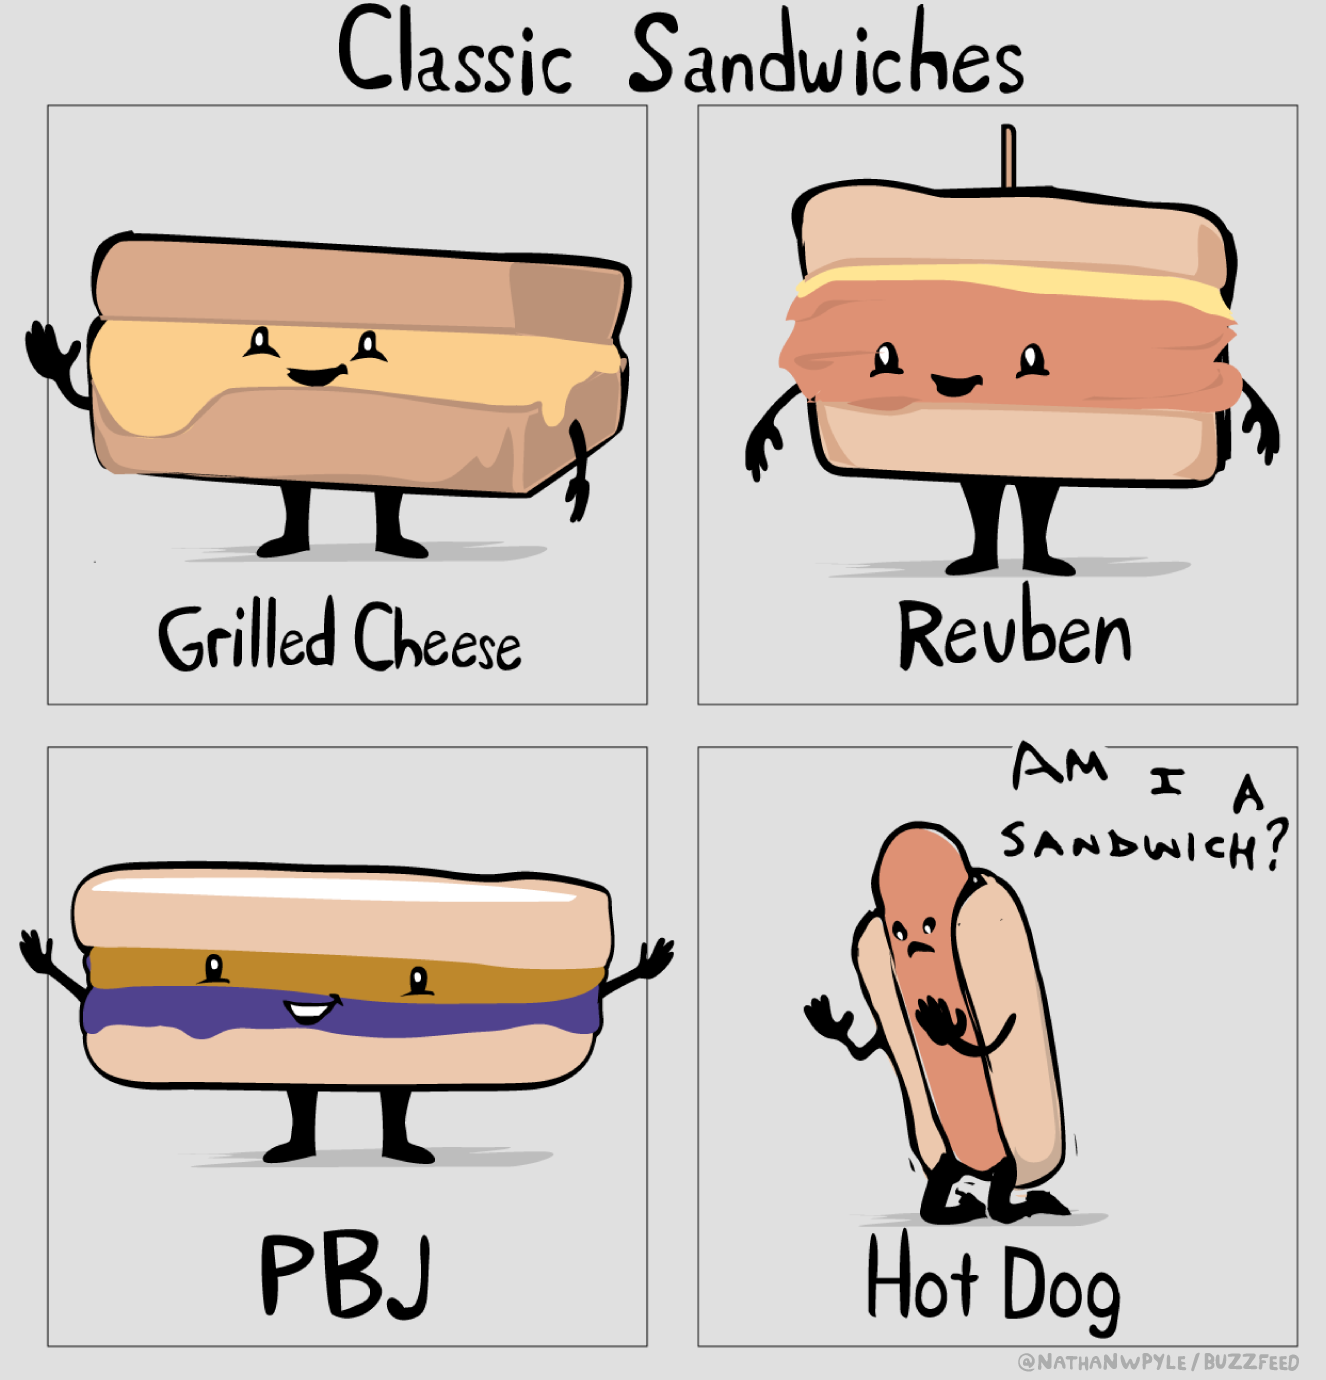
\includegraphics[width=0.5\textwidth]{hotdog_meme.png}
        % \label{fig:hotdog-meme} -- 0.6
        \caption{\label{fig:hotdog-meme}A hot dog experiencing existential dread \cite{imgur_classic_nodate}}
    \end{figure}
\end{frame}

\begin{frame}{The State of New York says ``Yes''!}
    \begin{figure}
        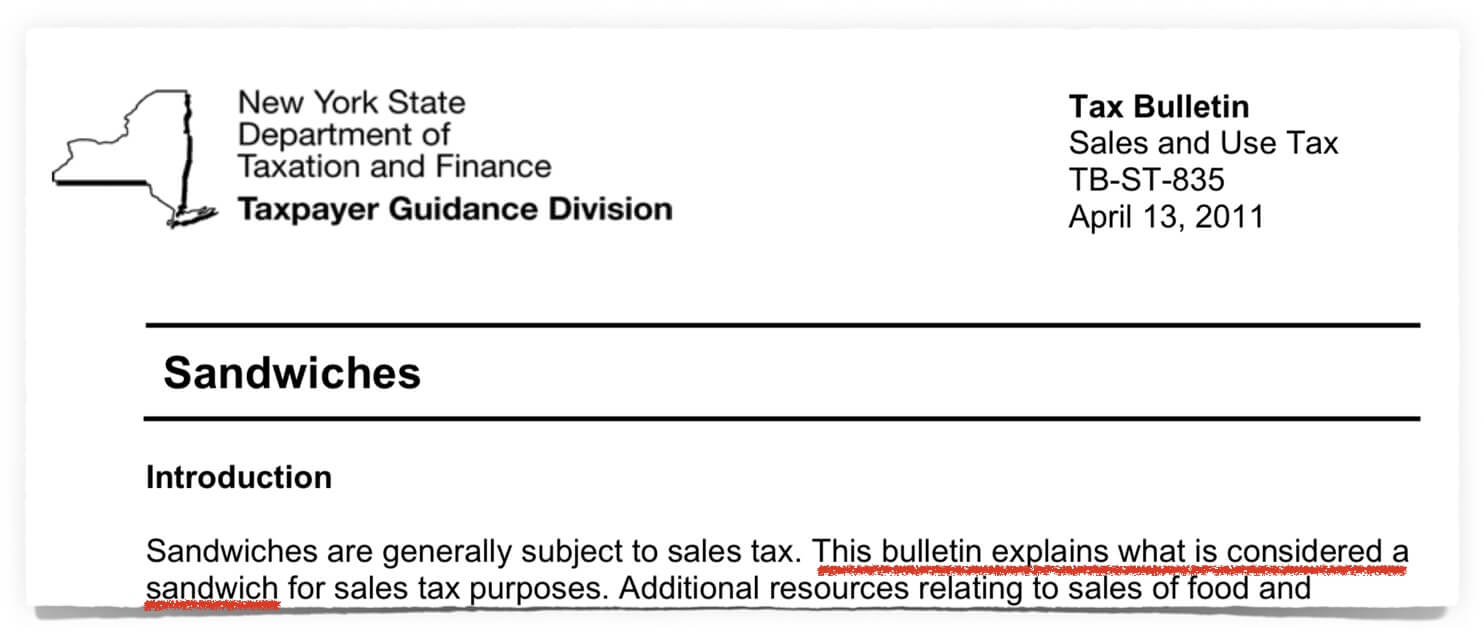
\includegraphics[width=0.65\textwidth]{ny_sandwich_law_1.jpg}
        \label{fig:ny-sandwich-law-top}
    \end{figure}
    \begin{figure}
        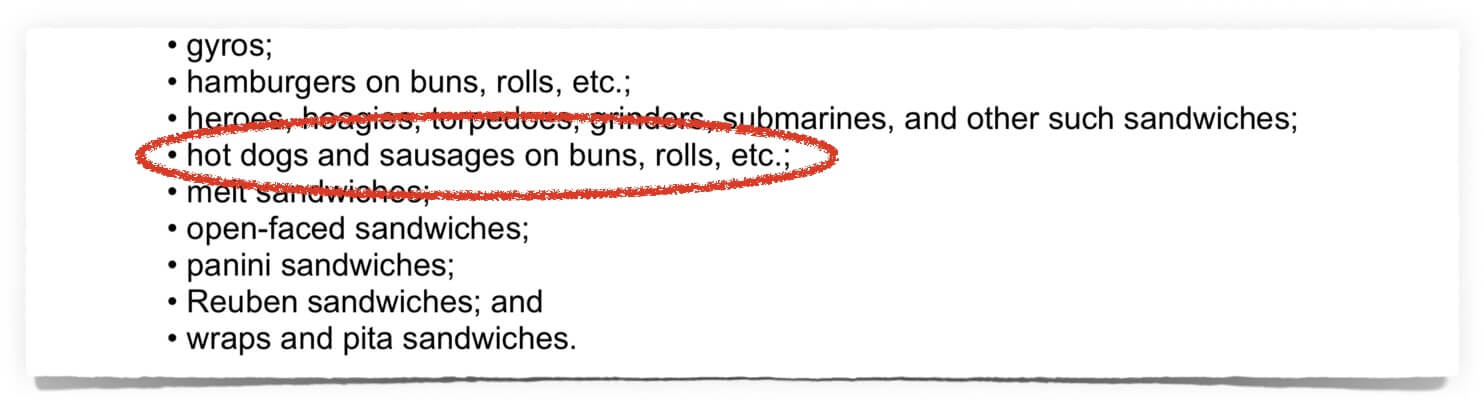
\includegraphics[width=0.8\textwidth]{ny_sandwich_law_2.jpg}
        \caption{\label{fig:ny-sandwich-law-bottom}New York State Tax Code classifying hot dogs as sandwiches}
    \end{figure}
\end{frame}

\begin{frame}{The ``Sandwich Alignment Chart'' attempted to bring order}
    \begin{figure}
        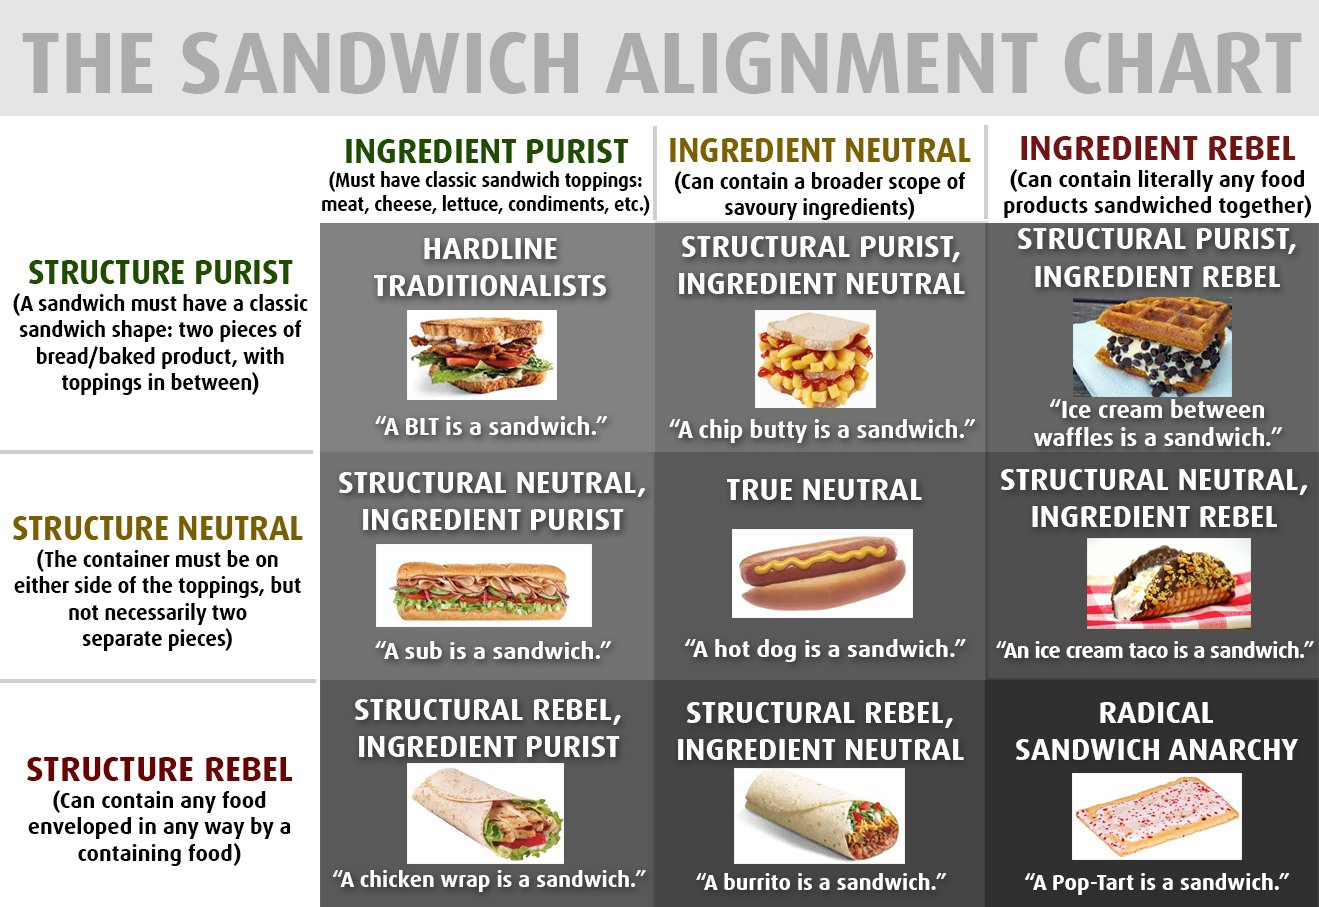
\includegraphics[width=0.75\textwidth]{sandwich_alignment.jpg}
        \caption{\label{fig:sandwich-alignment}An alignment chart for what is considered a sandwich \cite{noauthor_matttomic_nodate}}
    \end{figure}
\end{frame}

\begin{frame}{But this only led to more chaos...}
    \begin{figure}
        % \usepackage{graphicx, animate}
        % \animategraphics[width=0.5\textwidth,controls,loop,autoplay,scale=1]{0}{sandwich_chaos/slice_}{10}{9}
        \begin{subfigure}{.5\textwidth}
          \centering
          
\includegraphics[width=.8\linewidth]{sandwich_chaos/slice_6.png} %slice_0.png
          \label{fig:sandwich-chaos-left}
        \end{subfigure}%
        \begin{subfigure}{.5\textwidth}
          \centering
          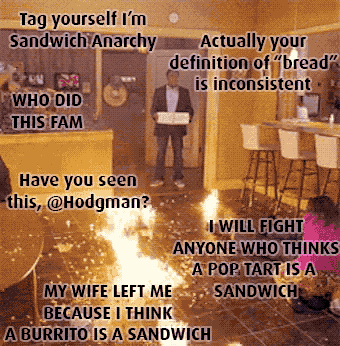
\includegraphics[width=.8\linewidth]{sandwich_chaos/slice_10.png}
          \label{fig:sandwich-chaos-right}
        \end{subfigure}
    \end{figure}
\end{frame}

\begin{frame}{Until @Phosphatide enlightened the world...}
    \begin{figure}
        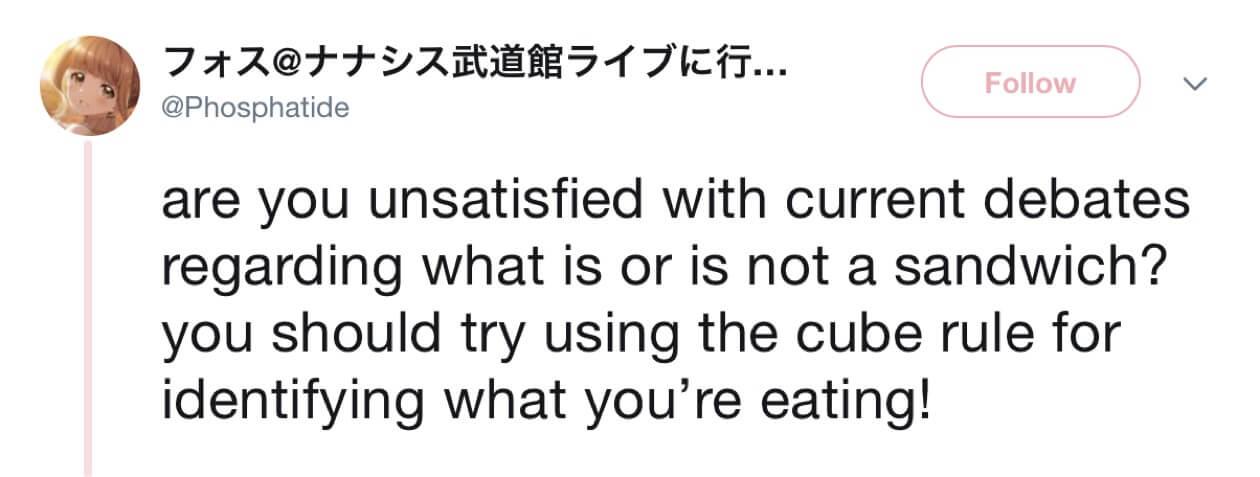
\includegraphics[width=0.9\textwidth]{phosphatide.jpg}
        \caption{\label{fig:phosphatide}A tweet introducing the ``Cube Rule of Food''\cite{noauthor_phosphatide_nodate}}
    \end{figure}
\end{frame}

\begin{frame}{The Cube Rule of Food}
    \begin{figure}
        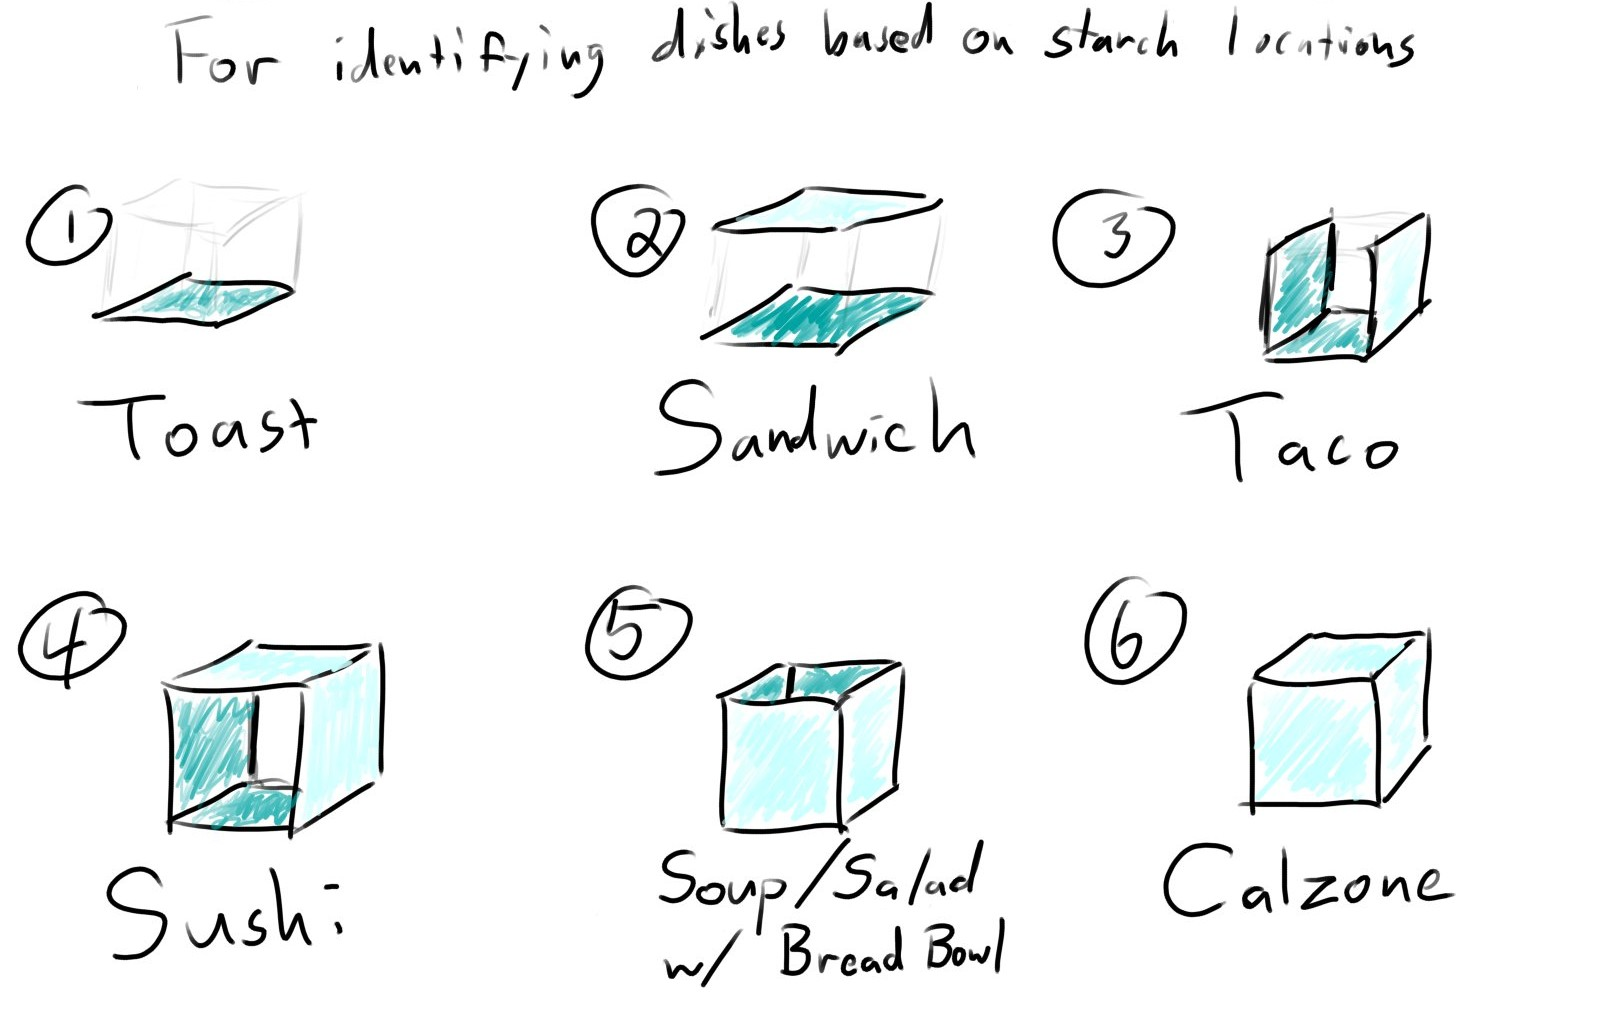
\includegraphics[width=0.9\textwidth]{cube_rule_of_food.jpg}
        \label{fig:cube-rule-of-food}
    \end{figure}
\end{frame}

\begin{frame}{The Cube Rule of Food}
    \begin{itemize}
        \item Two foodstuffs are isomorphic under the ``Cube Rule of Food'' iff the location of their starch content as mapped onto a cube are the same
        \vskip 0.5cm
        \item This partitions the set of all foodstuffs into equivalence classes based on the location of their starch content\footnote{Will need some additional special cases to cover the entire set}
        \begin{itemize}
            \item Foodstuffs can be referred to interchangeably within their equivalence class, for example: \textit{A slice of toast \textbf{is} Pizza}
        \end{itemize}
    \end{itemize}
\end{frame}

% Toast
\begin{frame}{The Cube Rule of Food -- Toast}
    \begin{figure}
        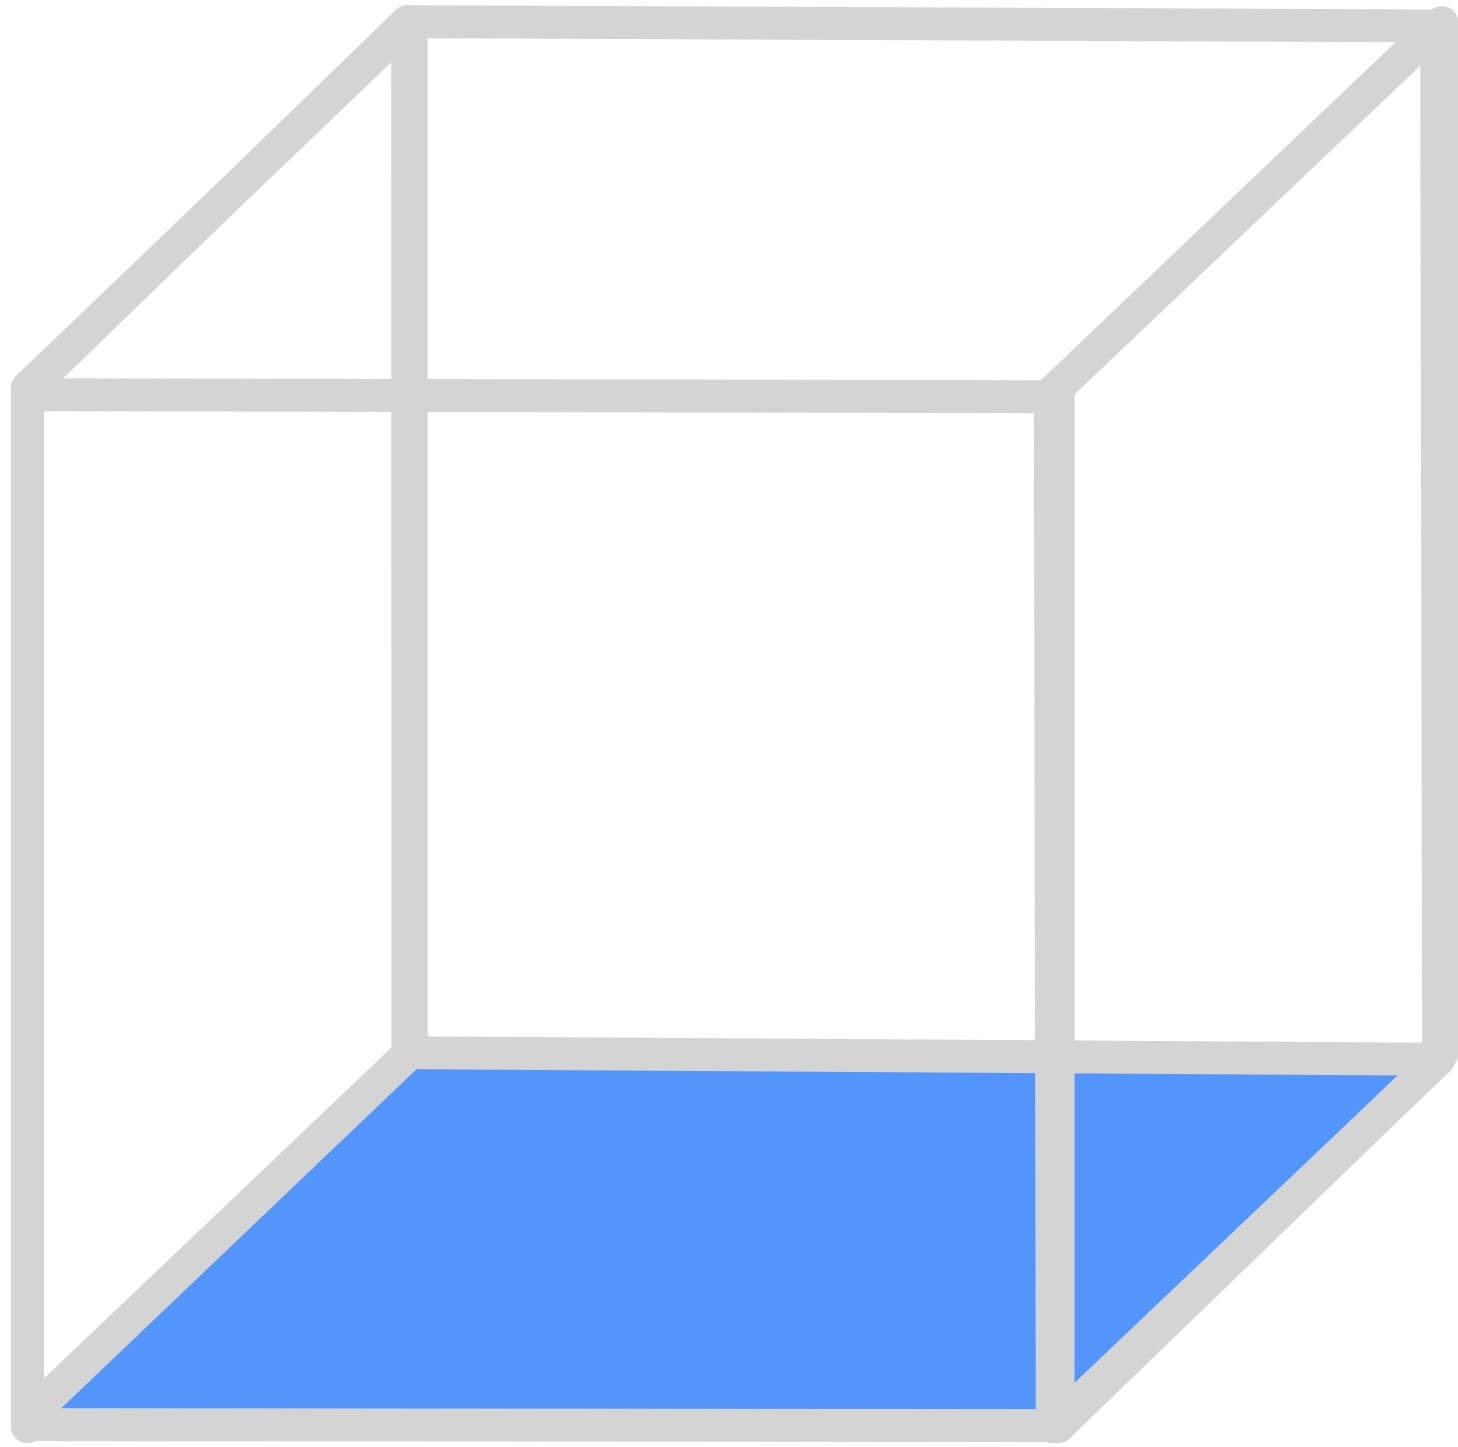
\includegraphics[width=0.5\textwidth]{toast/16_toast.jpg}
        \caption{\label{fig:toast-diagram}The starch locations of the ``Toast'' equivalence class}
    \end{figure}
\end{frame}

\begin{frame}{Examples of Toast}
    \begin{tikzpicture}[remember picture,overlay]
        \node[xshift=-1.1cm,yshift=-2cm] at (current page.north east) {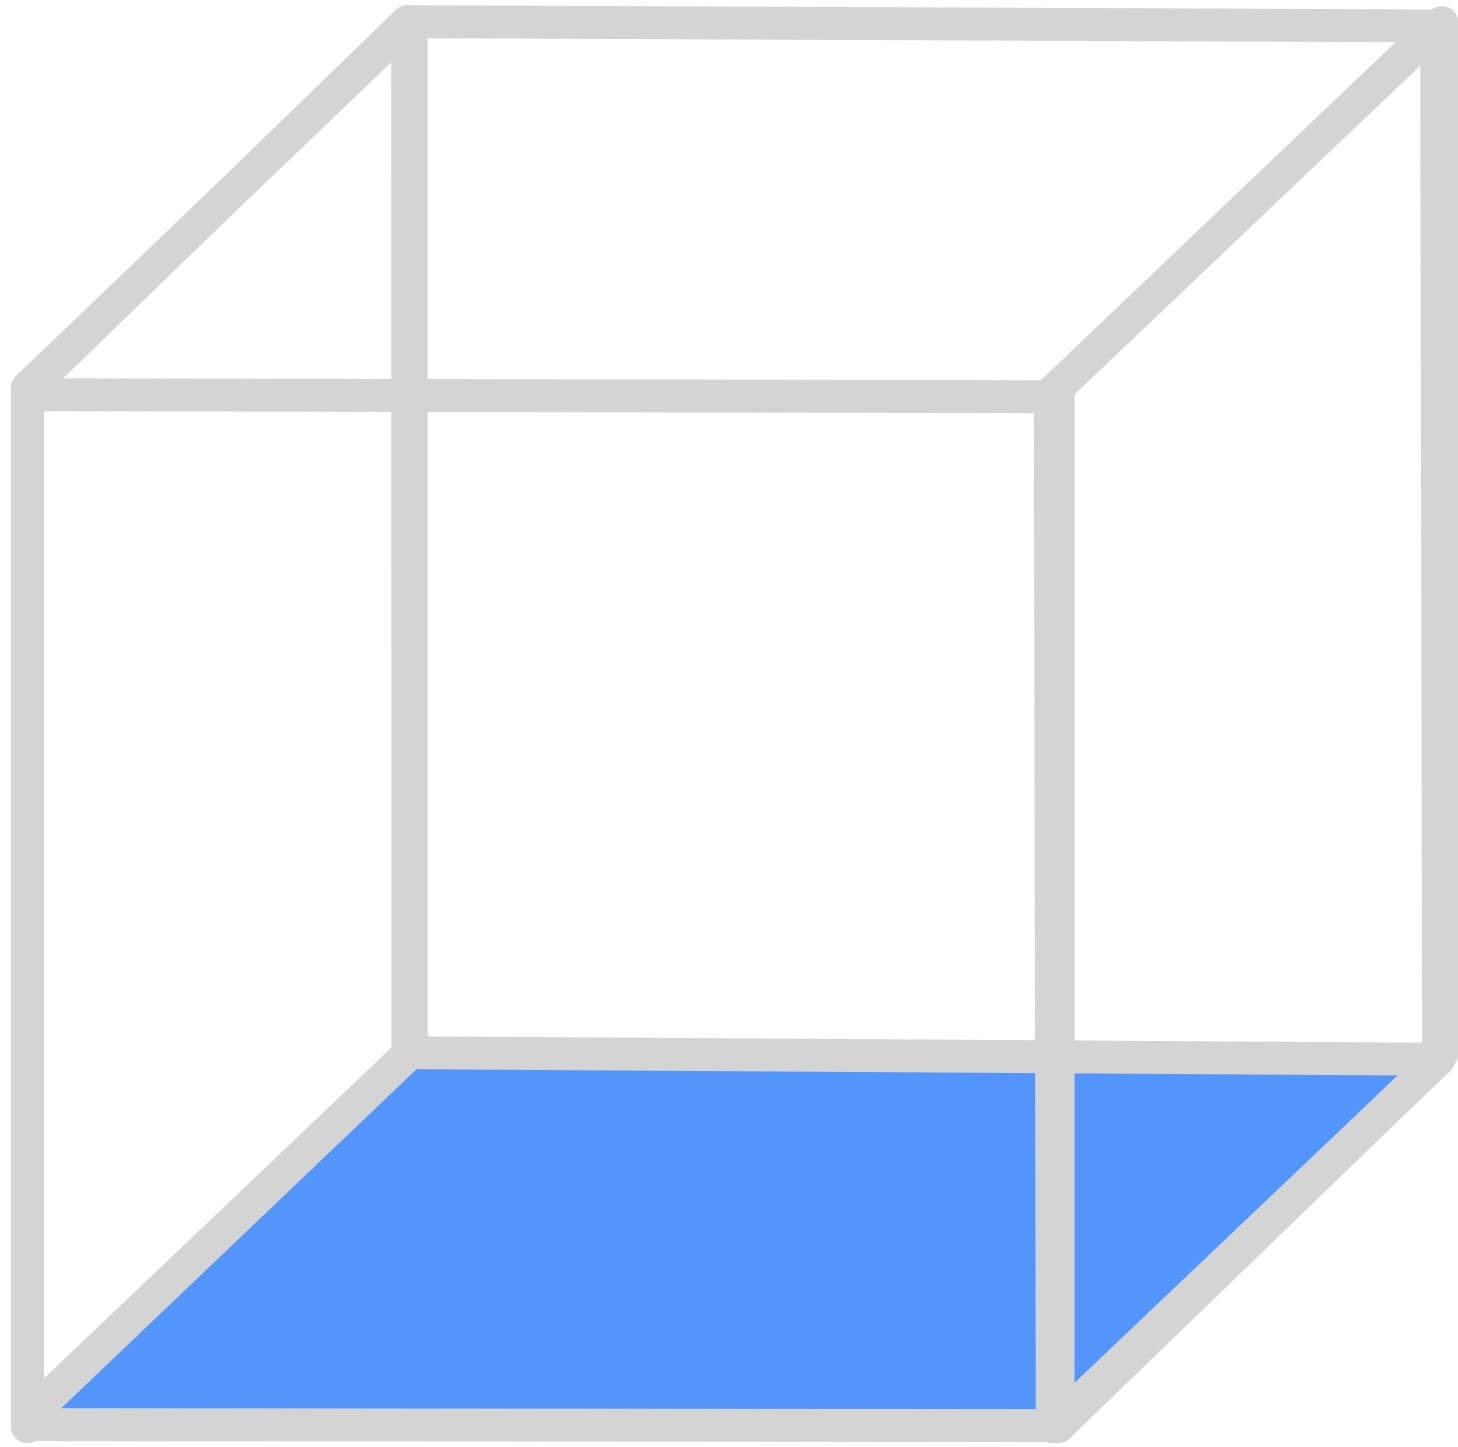
\includegraphics[width=0.1\textwidth]{toast/16_toast.jpg}};
        % \node[xshift=-1.1cm,yshift=1.3cm] at (current page.south east) {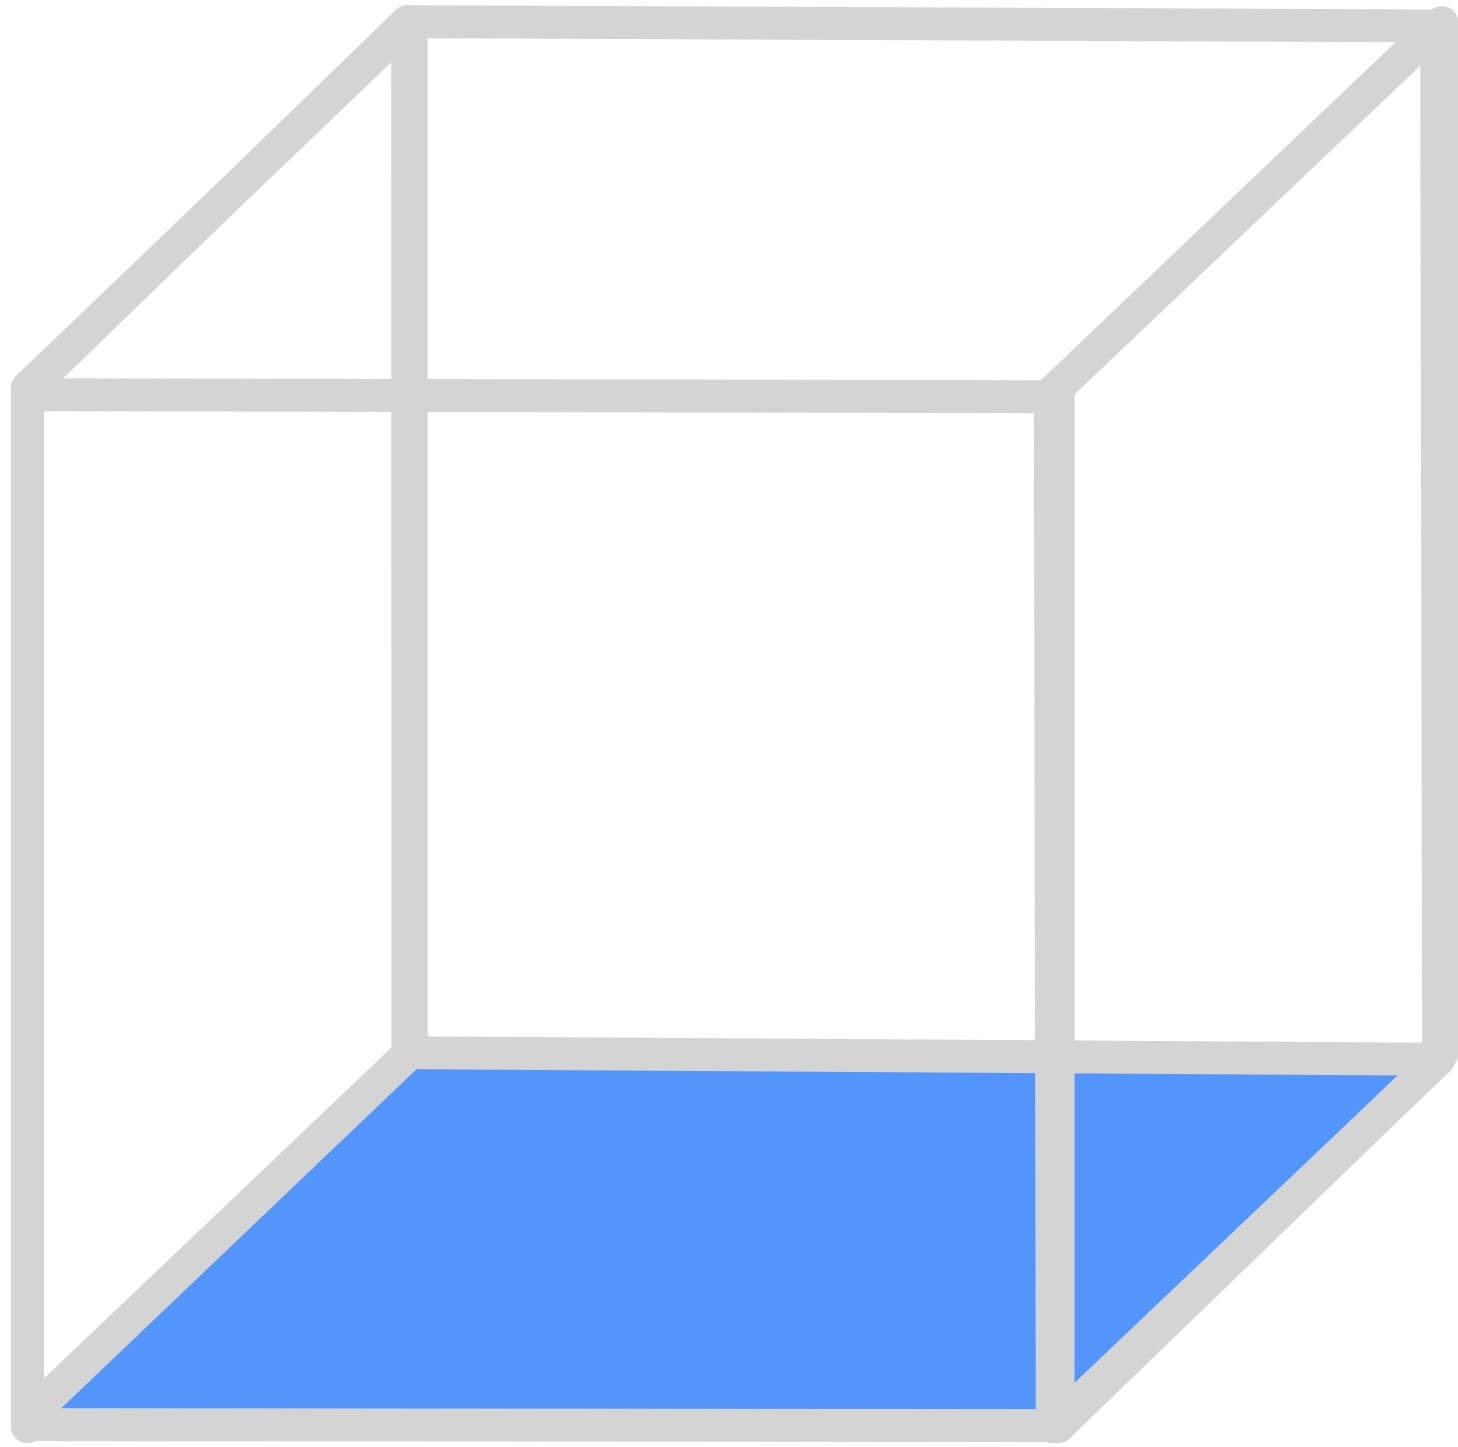
\includegraphics[width=0.1\textwidth]{toast/16_toast.jpg}};
    \end{tikzpicture}
    % \vskip 1cm
    \begin{figure}
        \begin{subfigure}{.4\textwidth}
          \centering
          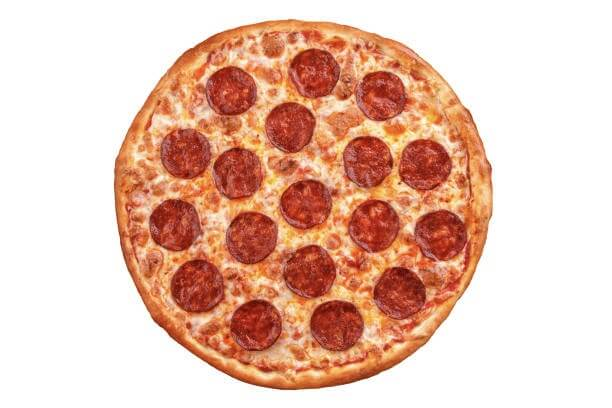
\includegraphics[width=.8\linewidth]{toast/17_pizza.jpg}
          \caption{\label{fig:pizza}Pizza}
        \end{subfigure}%
        \begin{subfigure}{.4\textwidth}
          \centering
          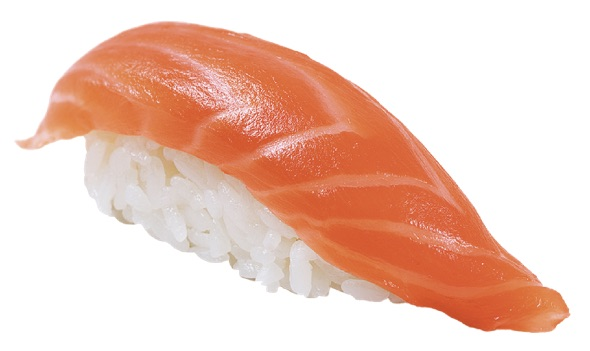
\includegraphics[width=.8\linewidth]{toast/17_nigiri.jpg}
          \caption{\label{fig:nigiri}Nigiri Sushi}
        \end{subfigure}
        \begin{subfigure}{.4\textwidth}
          \centering
          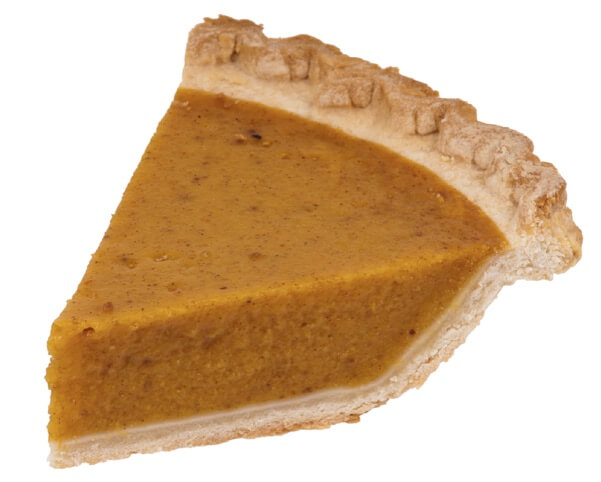
\includegraphics[width=.7\linewidth]{toast/17_pumpkin_pie_slice.jpg}
          \caption{\label{fig:pumpkin-pie}A slice of Pumpkin Pie\\\quad\quad(i.e. bent toast)}
        \end{subfigure}
    \end{figure}
\end{frame}


% Sandwich
\begin{frame}{The Cube Rule of Food -- Sandwich}
    \begin{figure}
        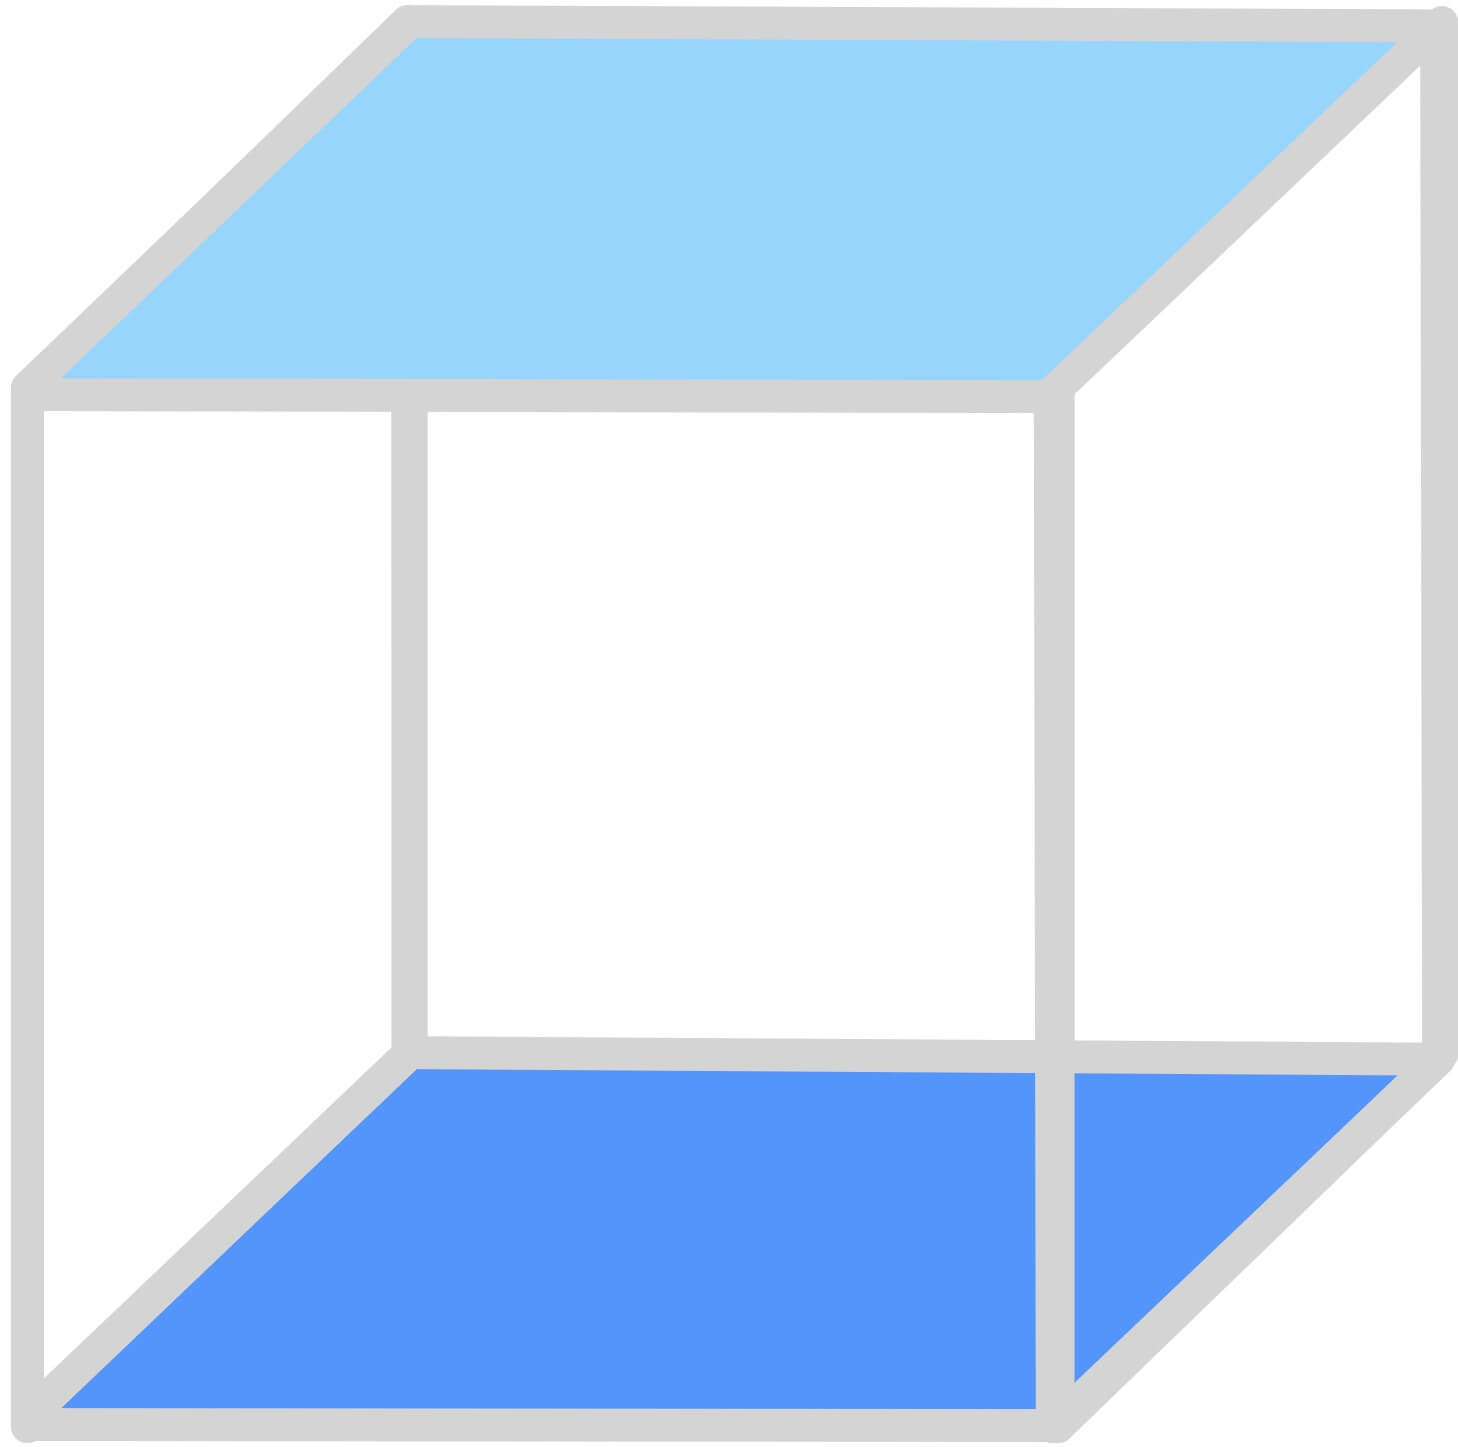
\includegraphics[width=0.5\textwidth]{sandwich/18_sandwich.jpg}
        \caption{\label{fig:sandwich-diagram}The starch locations of the ``Sandwich'' equivalence class}
    \end{figure}
\end{frame}

\begin{frame}{Examples of Sandwiches}
    \begin{tikzpicture}[remember picture,overlay]
        \node[xshift=-1.1cm,yshift=-2cm] at (current page.north east) {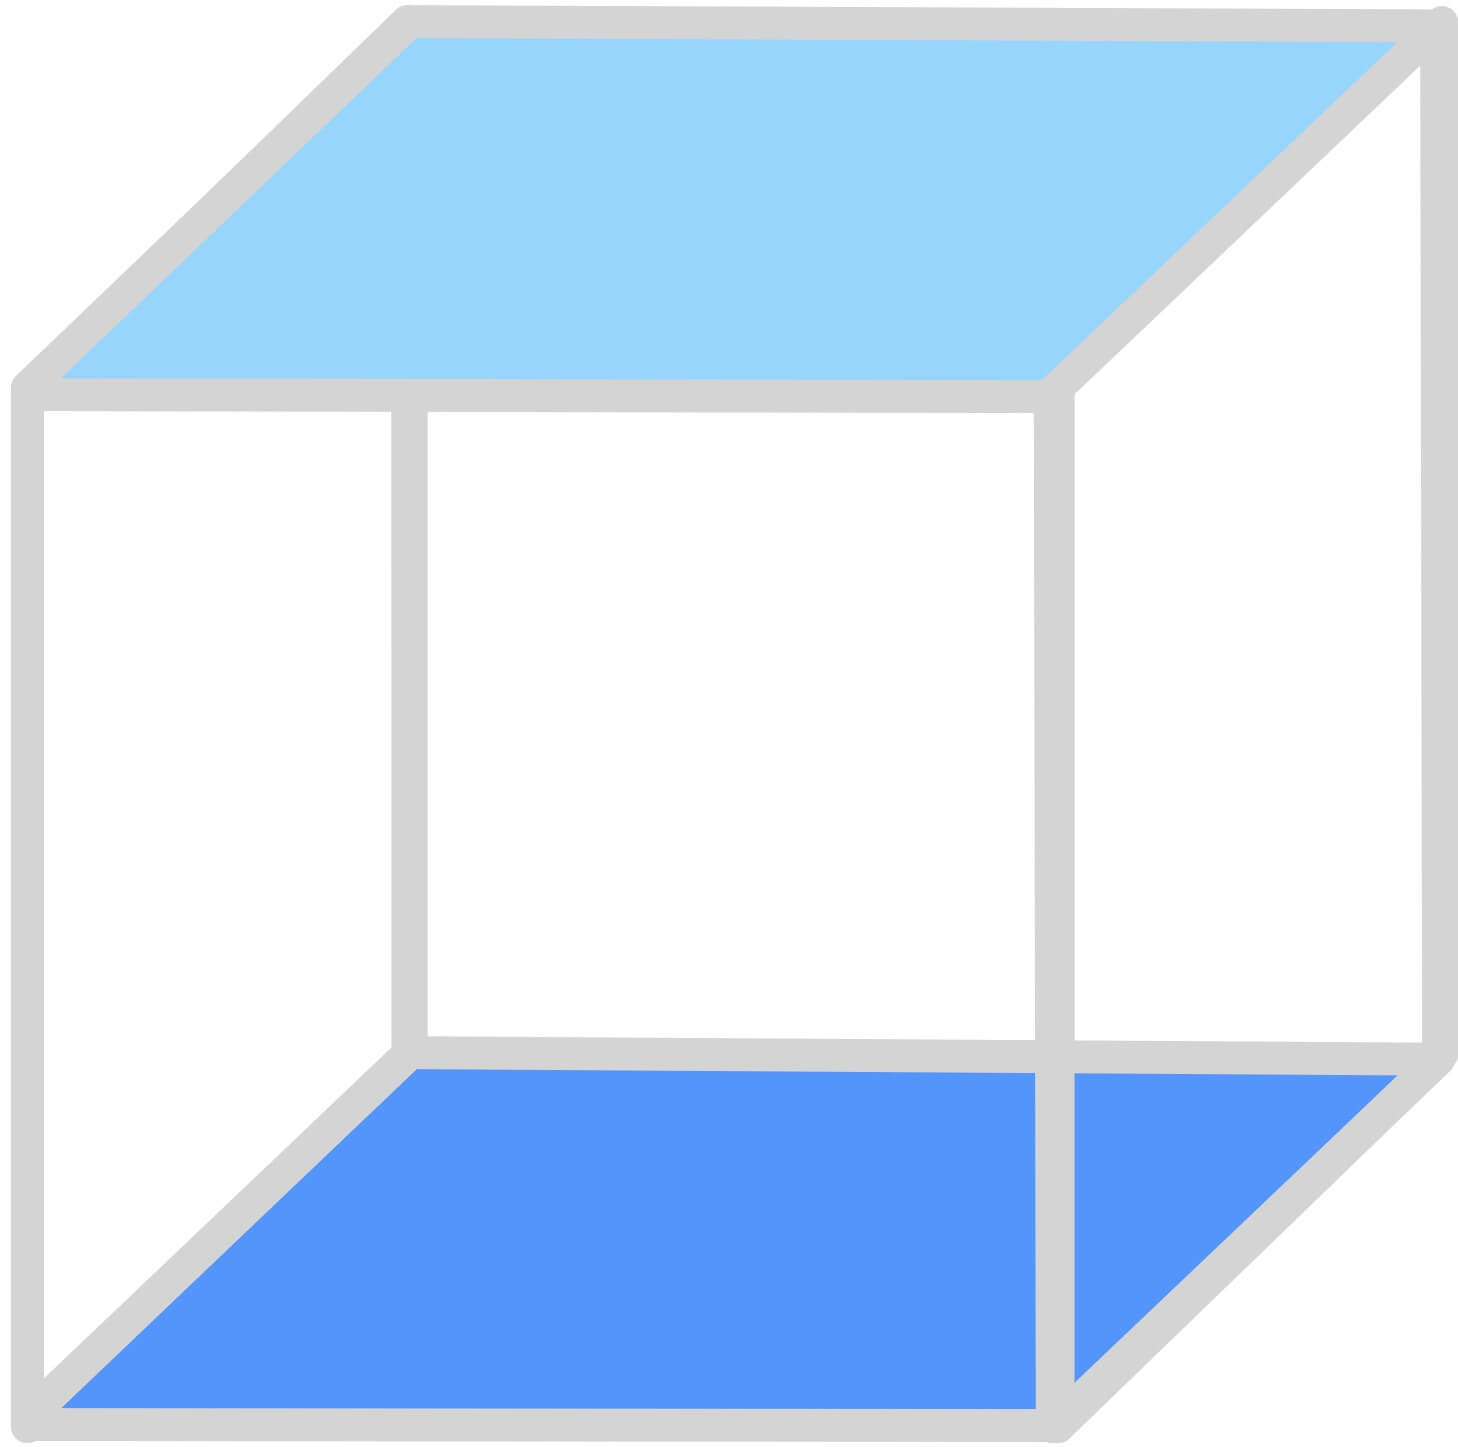
\includegraphics[width=0.1\textwidth]{sandwich/18_sandwich.jpg}};
    \end{tikzpicture}
    \begin{figure}
        \begin{subfigure}{.5\textwidth}
          \centering
          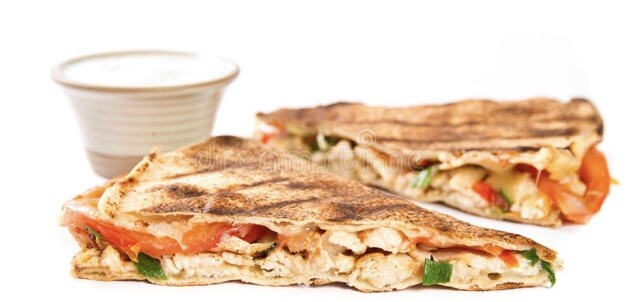
\includegraphics[width=\linewidth]{sandwich/19_quesadilla.jpg}
          \caption{\label{fig:quesadilla}Quesadilla}
        \end{subfigure}%
        \begin{subfigure}{.5\textwidth}
          \centering
          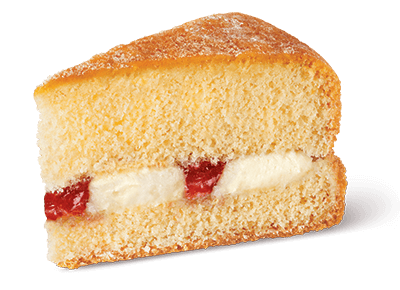
\includegraphics[width=.8\linewidth]{sandwich/19_victoria_sponge_cake.png}
          \caption{\label{fig:victoria-sponge}Victoria Sponge Cake}
        \end{subfigure}
    \end{figure}
\end{frame}

% Taco
\begin{frame}{The Cube Rule of Food -- Taco}
    \begin{figure}
        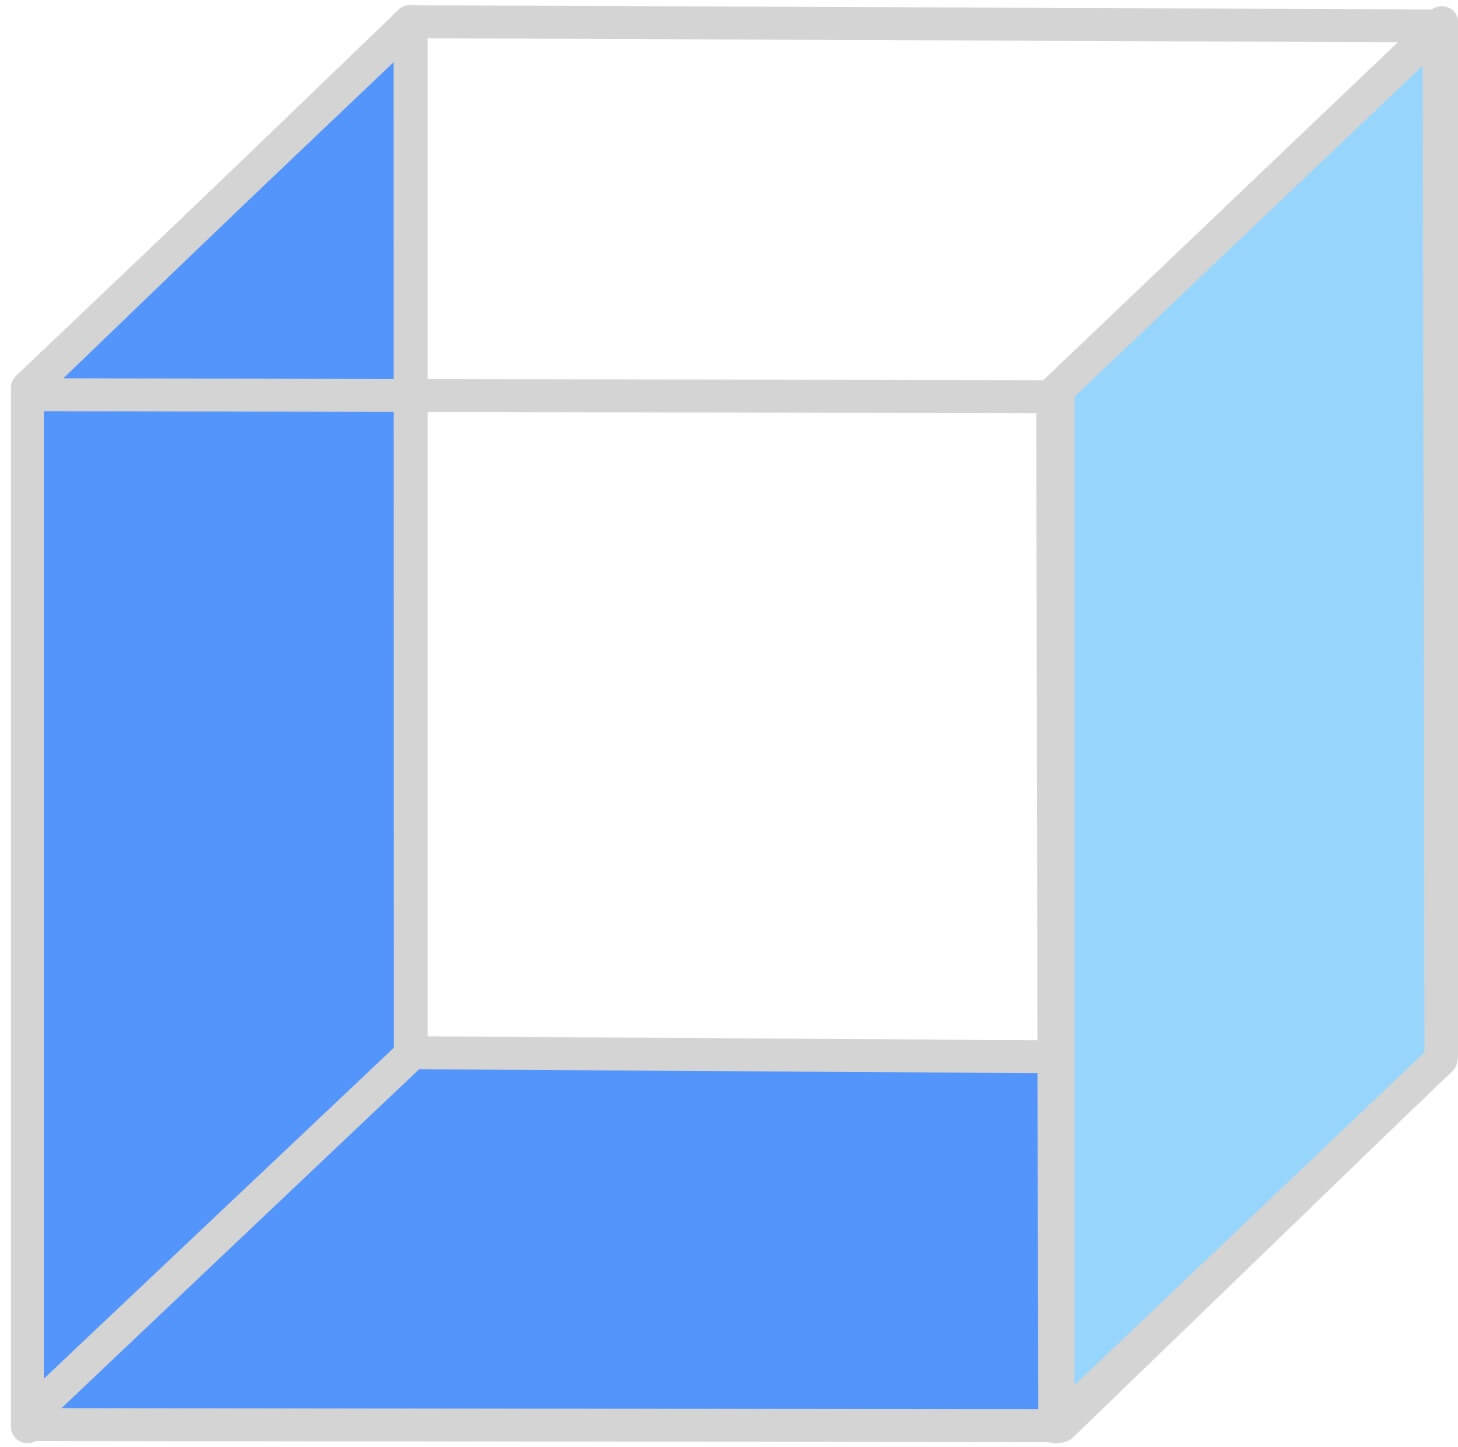
\includegraphics[width=0.5\textwidth]{taco/20_taco.jpg}
        \caption{\label{fig:taco-diagram}The starch locations of the ``Taco'' equivalence class}
    \end{figure}
\end{frame}

\begin{frame}{Examples of Tacos}
    \begin{tikzpicture}[remember picture,overlay]
        \node[xshift=-1.1cm,yshift=-2cm] at (current page.north east) {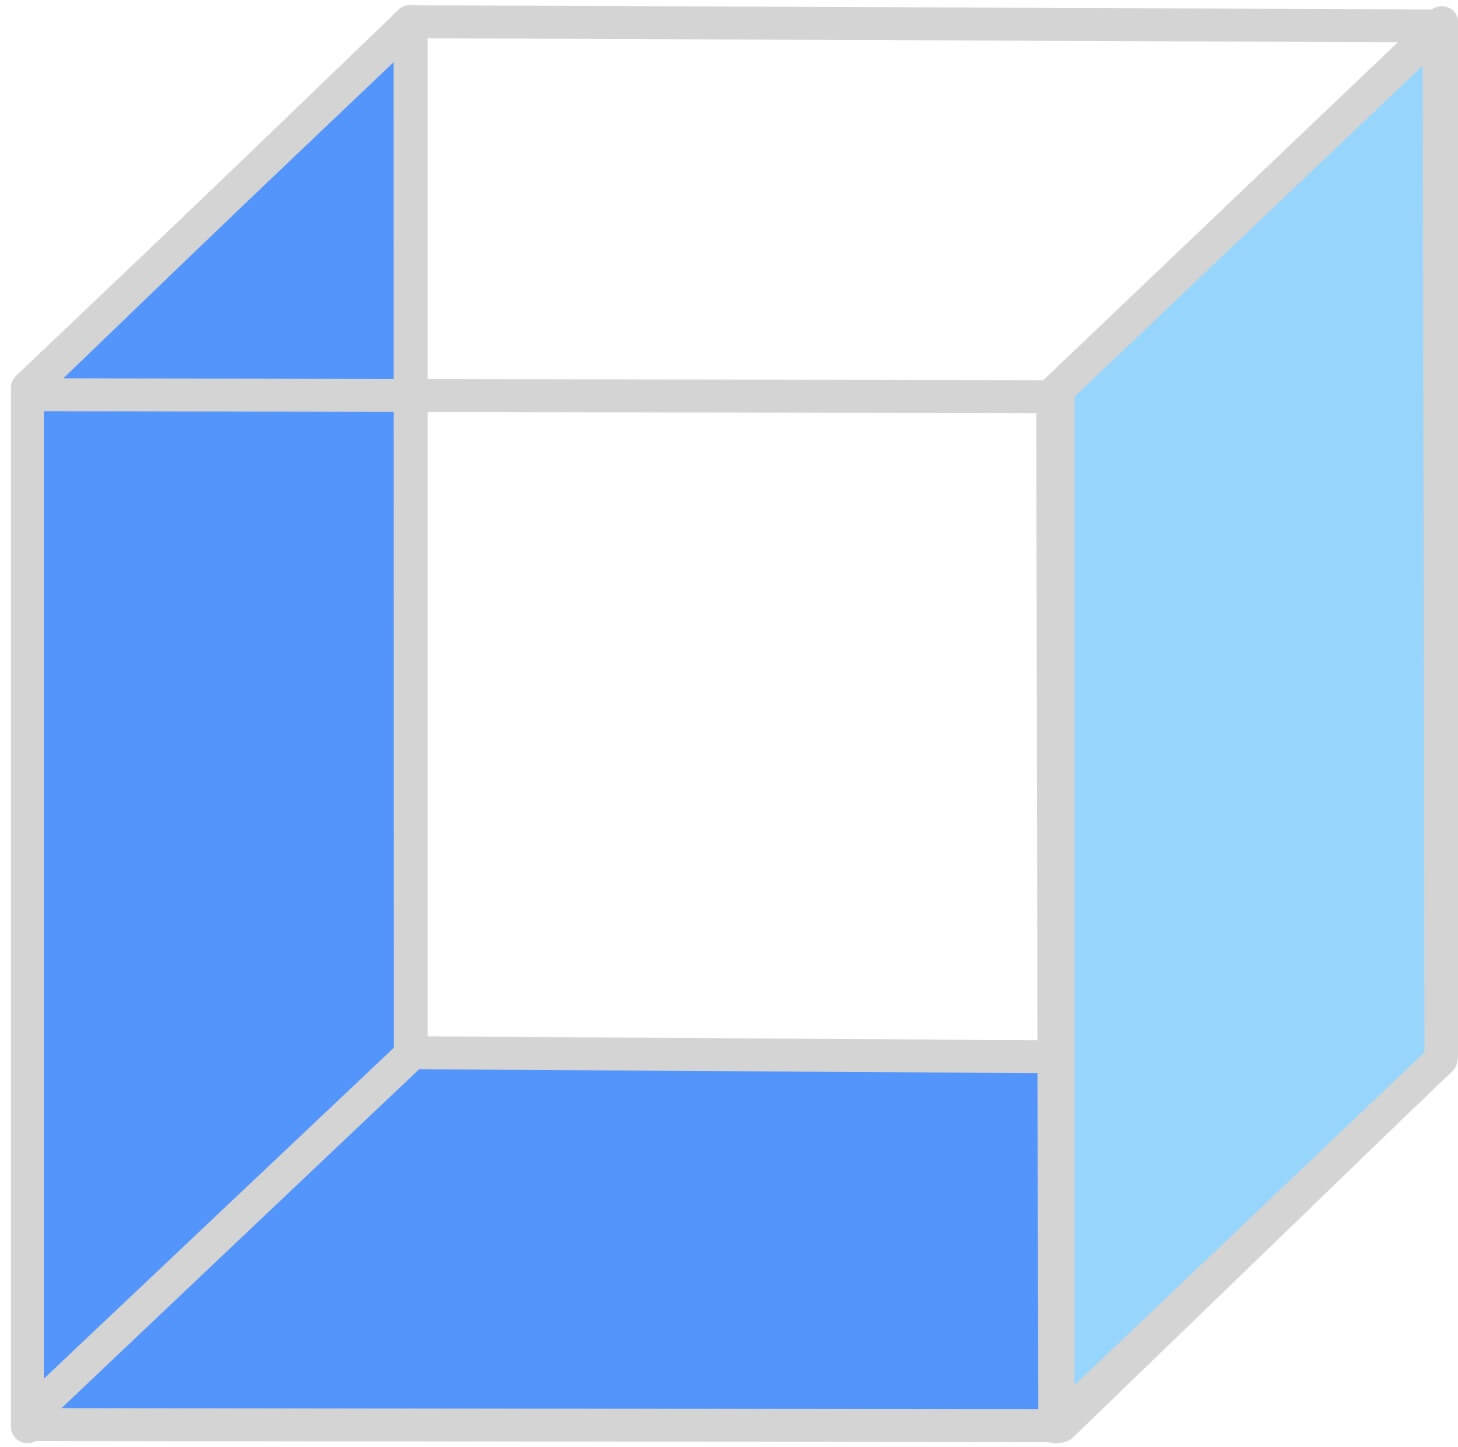
\includegraphics[width=0.1\textwidth]{taco/20_taco.jpg}};
    \end{tikzpicture}
    \begin{figure}
        \begin{subfigure}{.4\textwidth}
          \centering
          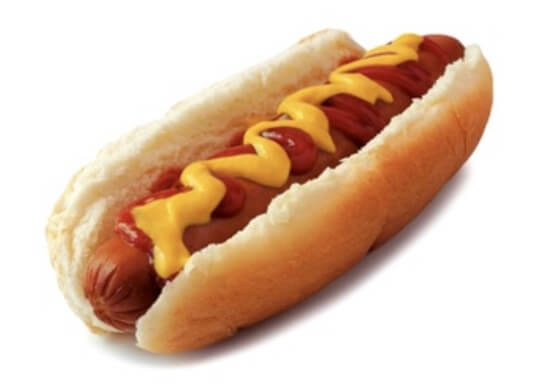
\includegraphics[width=.8\linewidth]{taco/20_hotdog.jpg}
          \caption{\label{fig:hot-dog-taco}Hot dog}
        \end{subfigure}%
        \begin{subfigure}{.4\textwidth}
          \centering
          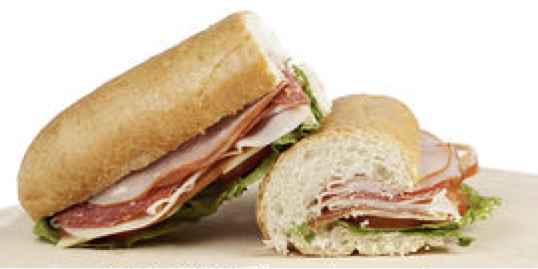
\includegraphics[width=.8\linewidth]{taco/20_sub.jpg}
          \caption{\label{fig:sub}Sub sandwich (uncut)}
        \end{subfigure}
        \begin{subfigure}{.5\textwidth}
          \centering
          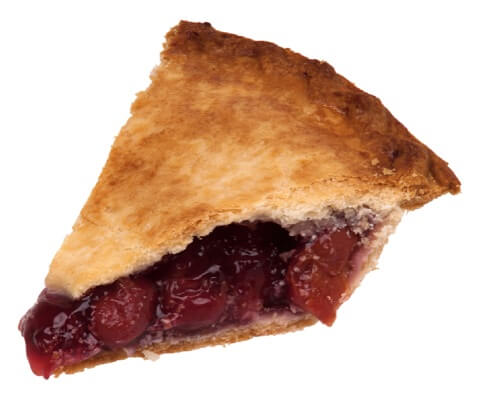
\includegraphics[width=.6\linewidth]{taco/20_pie_slice.jpg}
          \caption{\label{fig:pie-slices}A slice of pie (a taco on its side)}
        \end{subfigure}
    \end{figure}
\end{frame}

% Sushi
\begin{frame}{The Cube Rule of Food -- Sushi}
    \begin{figure}
        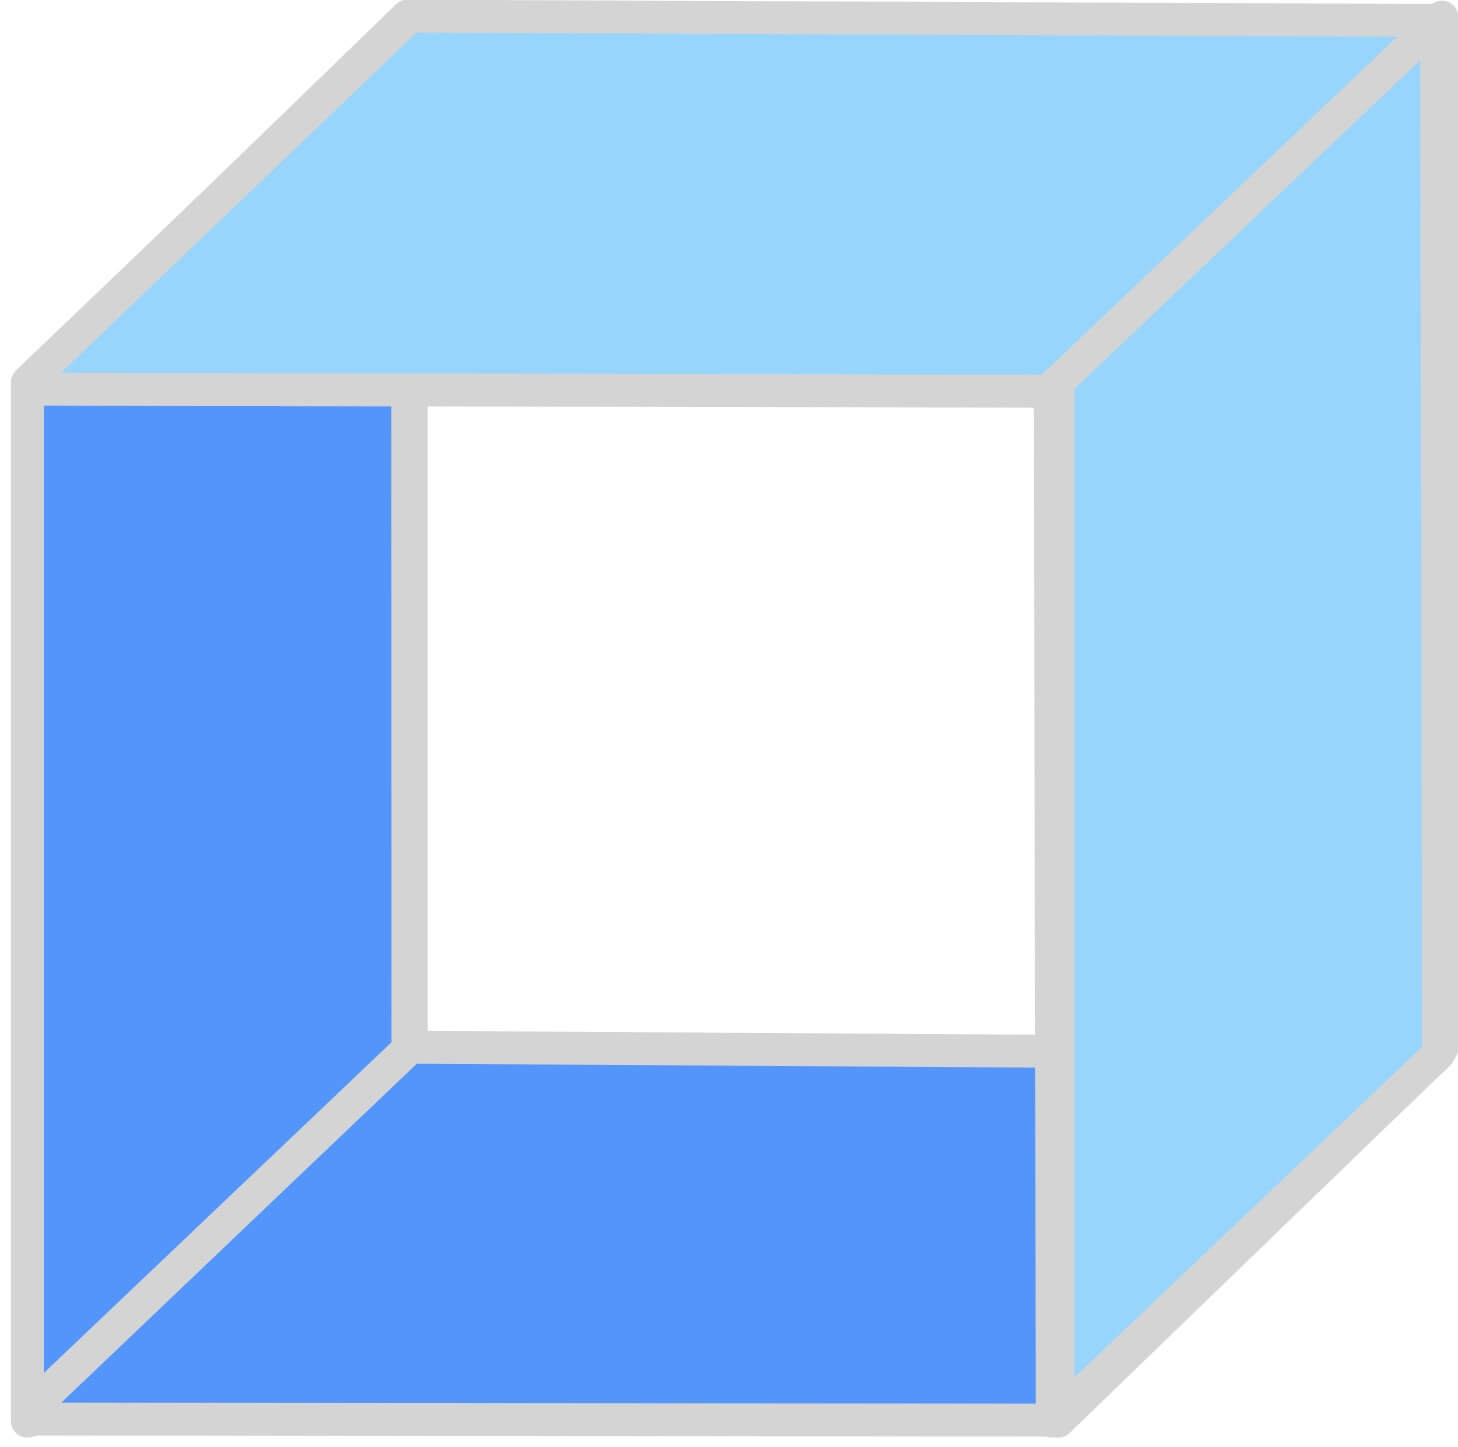
\includegraphics[width=0.5\textwidth]{sushi/21_sushi.jpg}
        \caption{\label{fig:sushi-diagram}The starch locations of the ``Sushi'' equivalence class}
    \end{figure}
\end{frame}

\begin{frame}{Examples of Sushi}
    \begin{tikzpicture}[remember picture,overlay]
        \node[xshift=-1.1cm,yshift=-2cm] at (current page.north east) {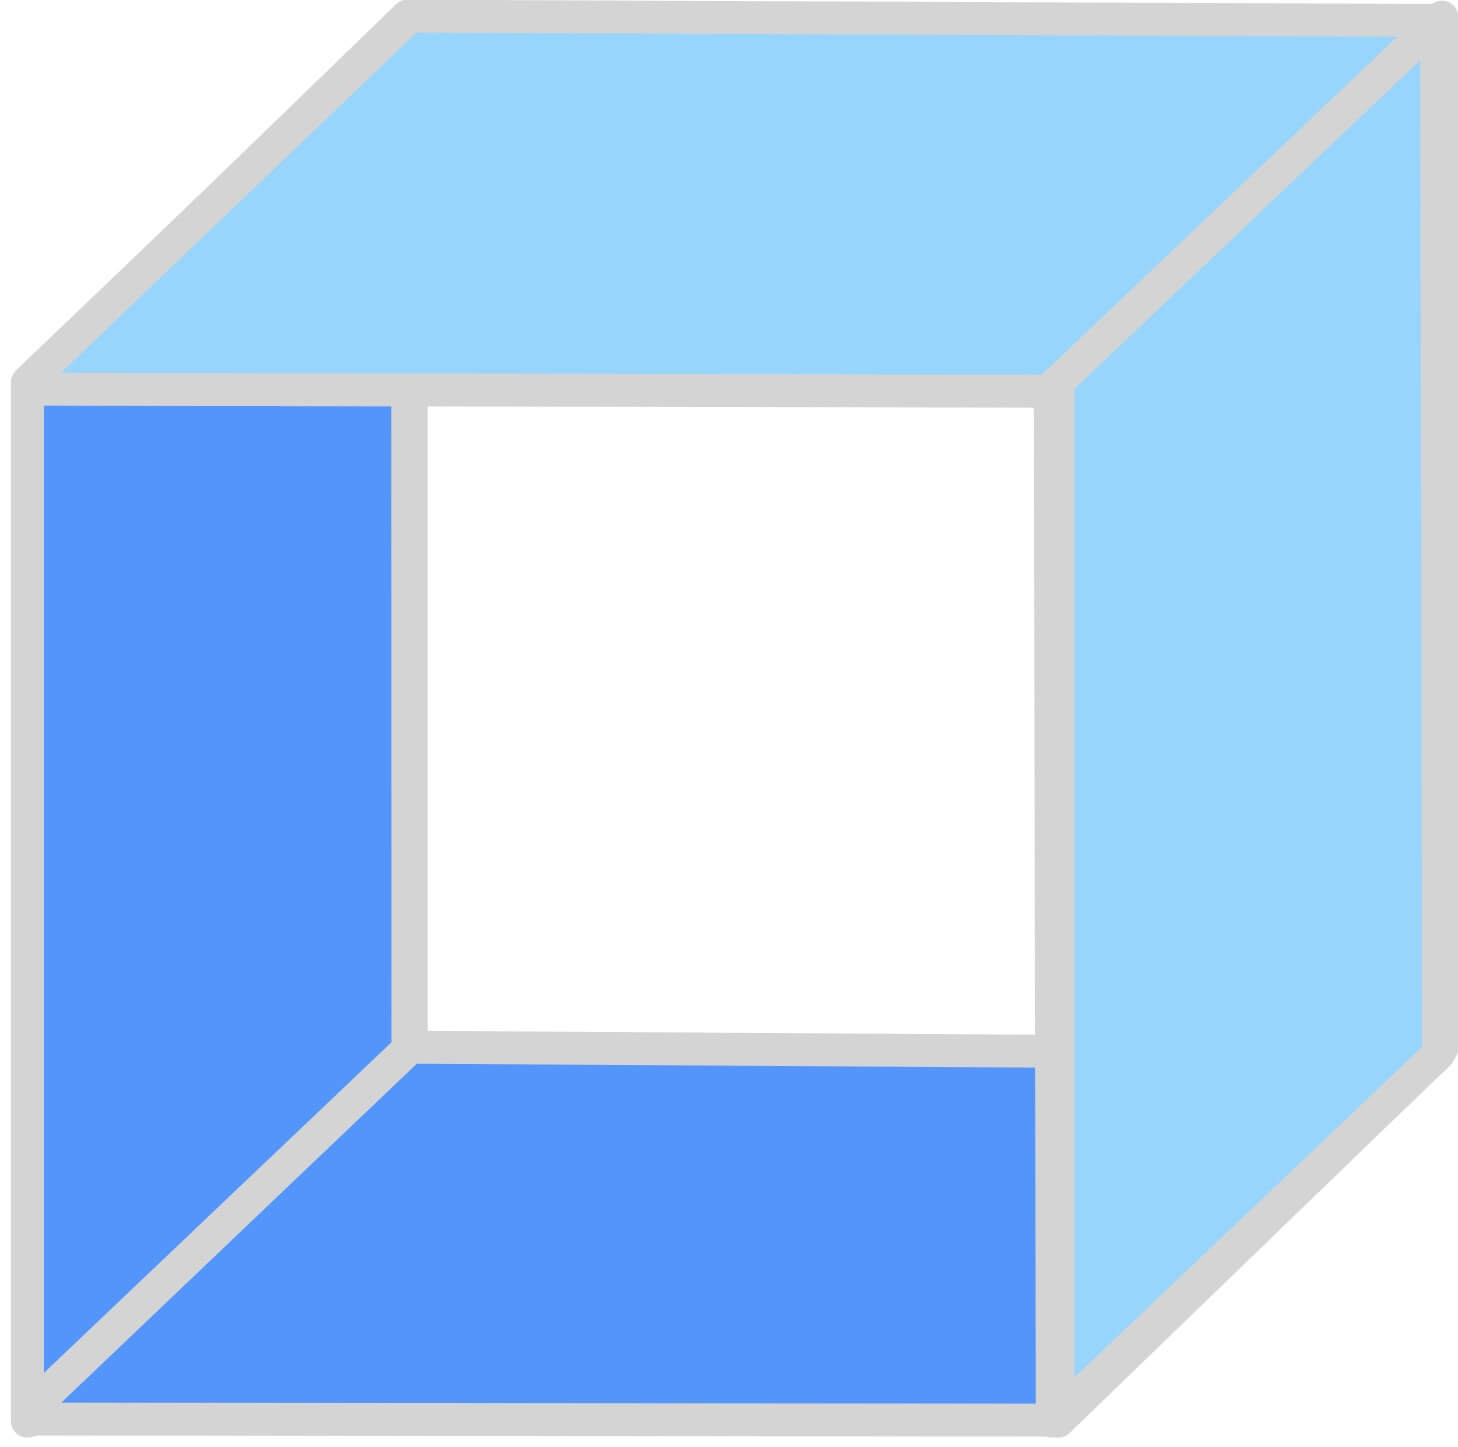
\includegraphics[width=0.1\textwidth]{sushi/21_sushi.jpg}};
    \end{tikzpicture}
    \begin{figure}
        \begin{subfigure}{.4\textwidth}
          \centering
          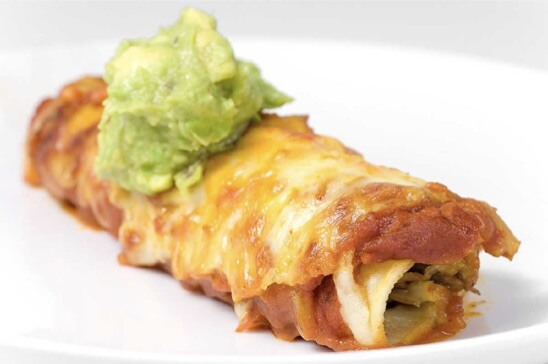
\includegraphics[width=.8\linewidth]{sushi/22_enchilada.jpg}
          \caption{\label{fig:enchilada}Enchilada}
        \end{subfigure}
        \begin{subfigure}{.4\textwidth}
          \centering
          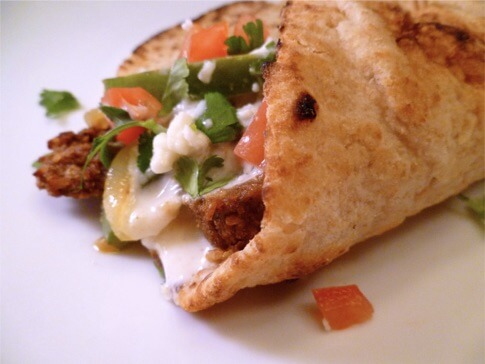
\includegraphics[width=.8\linewidth]{sushi/22_falafel.jpg}
          \caption{\label{fig:falafel}Falafel}
        \end{subfigure}%
        \begin{subfigure}{.4\textwidth}
          \centering
          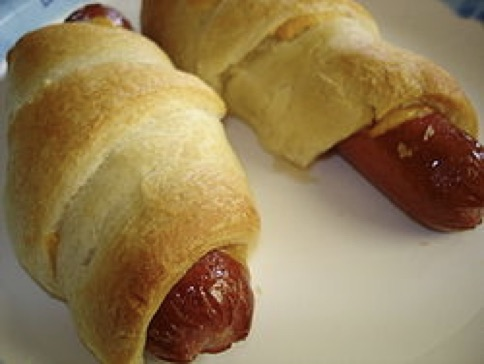
\includegraphics[width=.8\linewidth]{sushi/22_pigs.jpg}
          \caption{\label{fig:pigs-in-blankets}Pigs in blankets}
        \end{subfigure}
    \end{figure}
\end{frame}

% Quiche
\begin{frame}{The Cube Rule of Food -- Quiche}
    \begin{figure}
        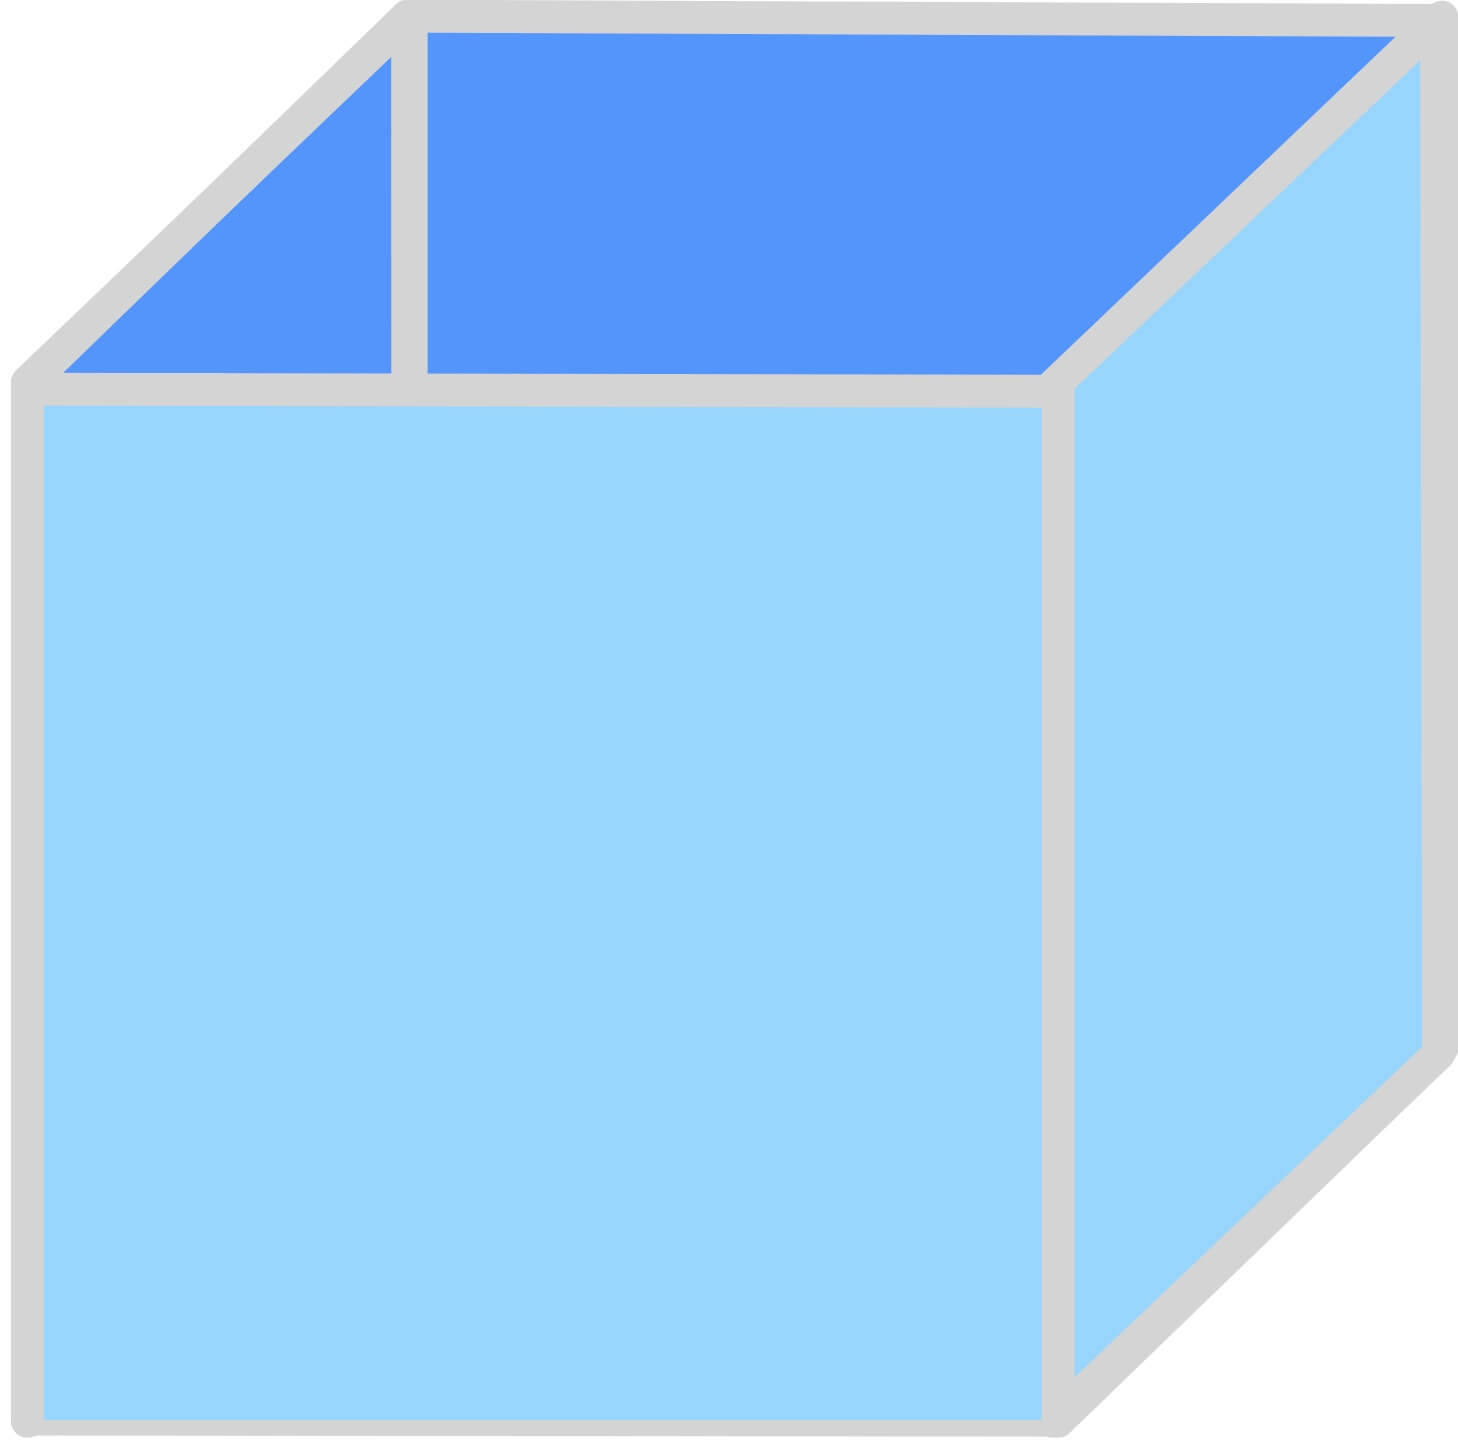
\includegraphics[width=0.5\textwidth]{quiche/23_quiche.jpg}
        \caption{\label{fig:quiche-diagram}The starch locations of the ``Quiche'' equivalence class}
    \end{figure}
\end{frame}

\begin{frame}{Examples of Quiche}
    \begin{tikzpicture}[remember picture,overlay]
        \node[xshift=-1.1cm,yshift=-2cm] at (current page.north east) {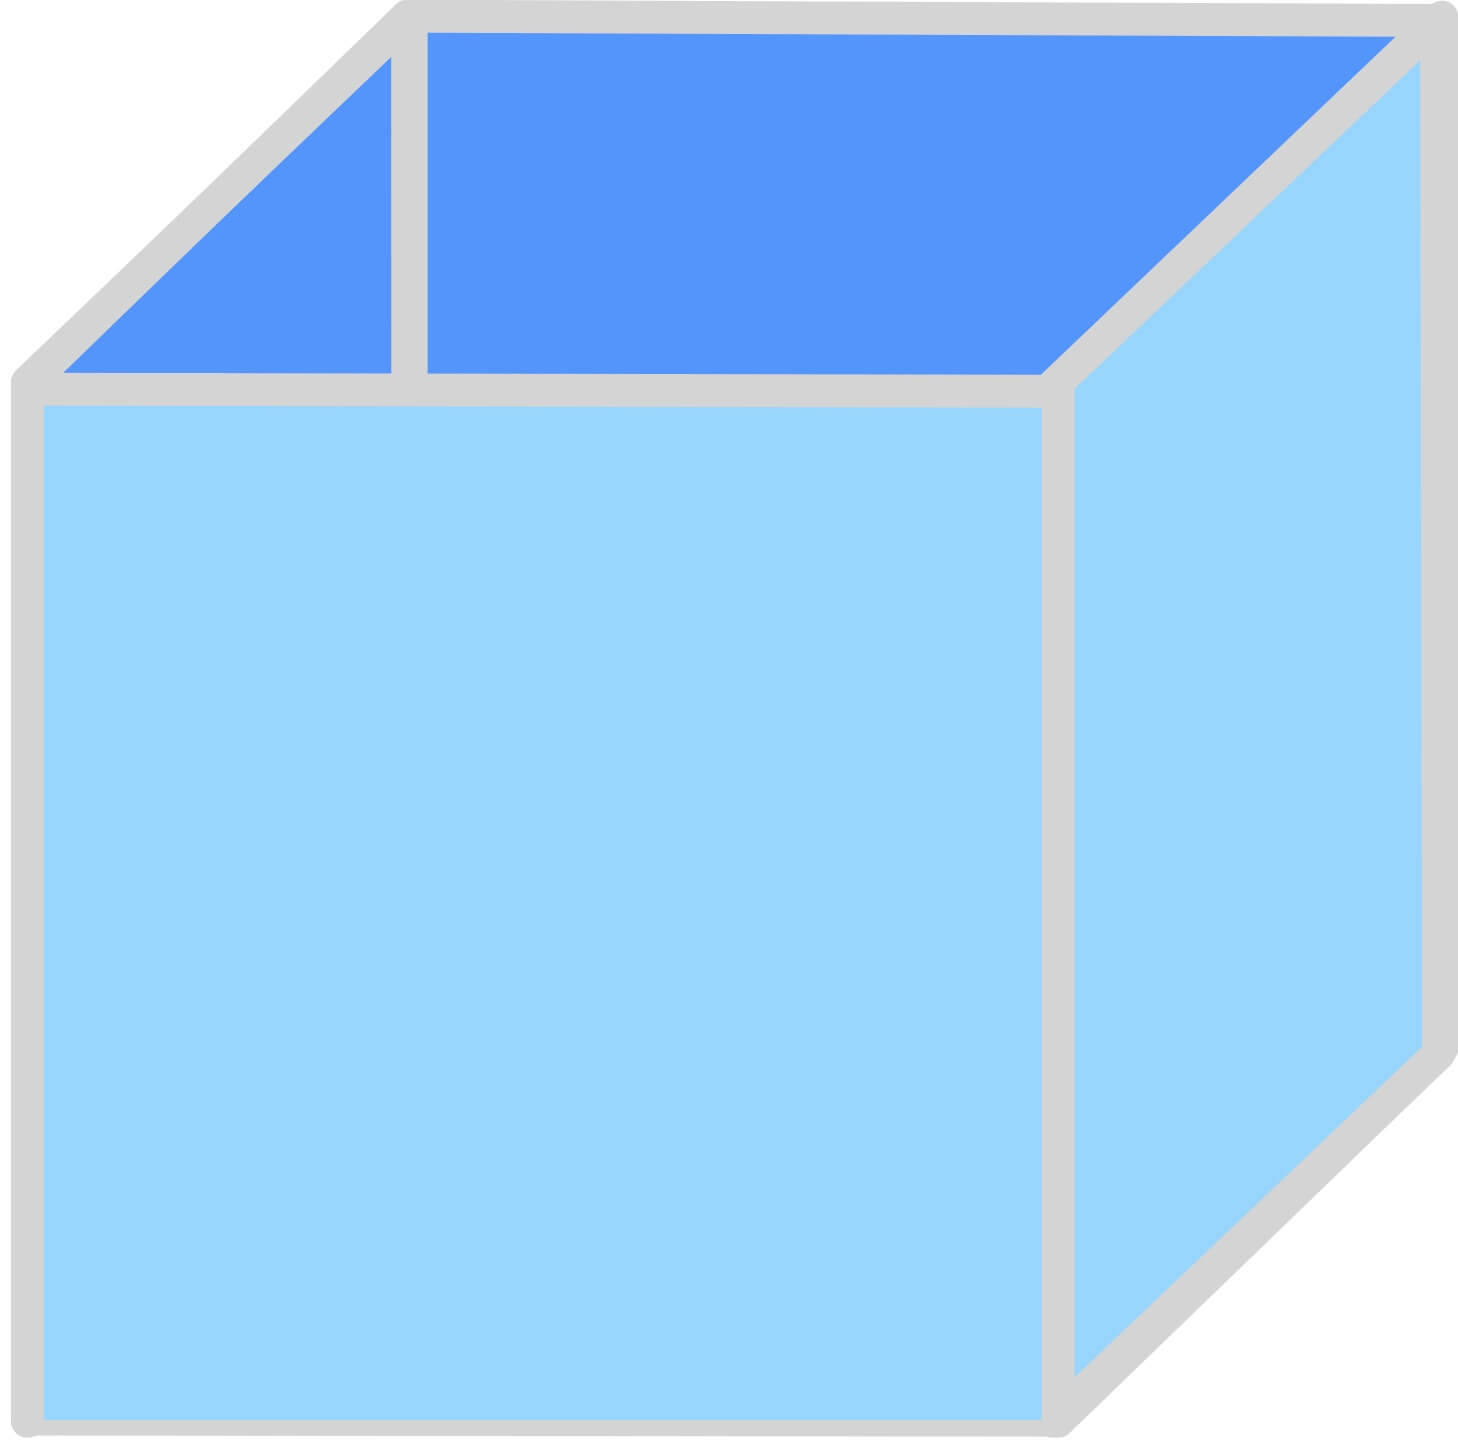
\includegraphics[width=0.1\textwidth]{quiche/23_quiche.jpg}};
    \end{tikzpicture}
    \begin{figure}
        \begin{subfigure}{.4\textwidth}
          \centering
          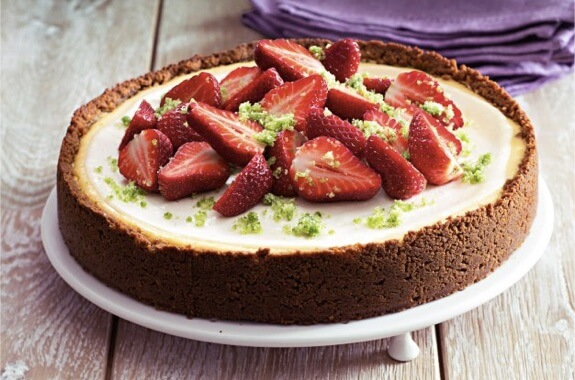
\includegraphics[width=.8\linewidth]{quiche/24_cheesecake.jpg}
          \caption{\label{fig:cheesecake}Cheesecake}
        \end{subfigure}
        \begin{subfigure}{.4\textwidth}
          \centering
          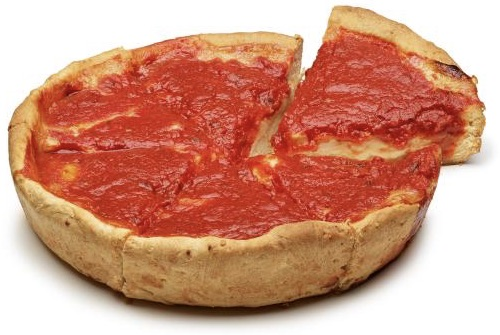
\includegraphics[width=.8\linewidth]{quiche/25_deep_dish.jpg}
          \caption{\label{fig:deep-dish}Deep dish pizza}
        \end{subfigure}%
        \begin{subfigure}{.4\textwidth}
          \centering
          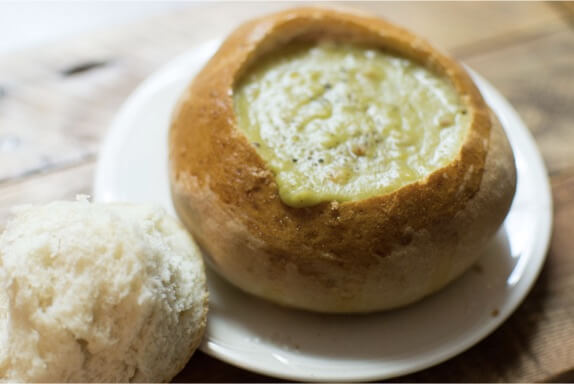
\includegraphics[width=.8\linewidth]{quiche/24_soup_bread_bowl.jpg}
          \caption{\label{fig:soup-bread-bowl}Soup bread bowl}
        \end{subfigure}
    \end{figure}
\end{frame}

% Calzone
\begin{frame}{The Cube Rule of Food -- Calzone}
    \begin{figure}
        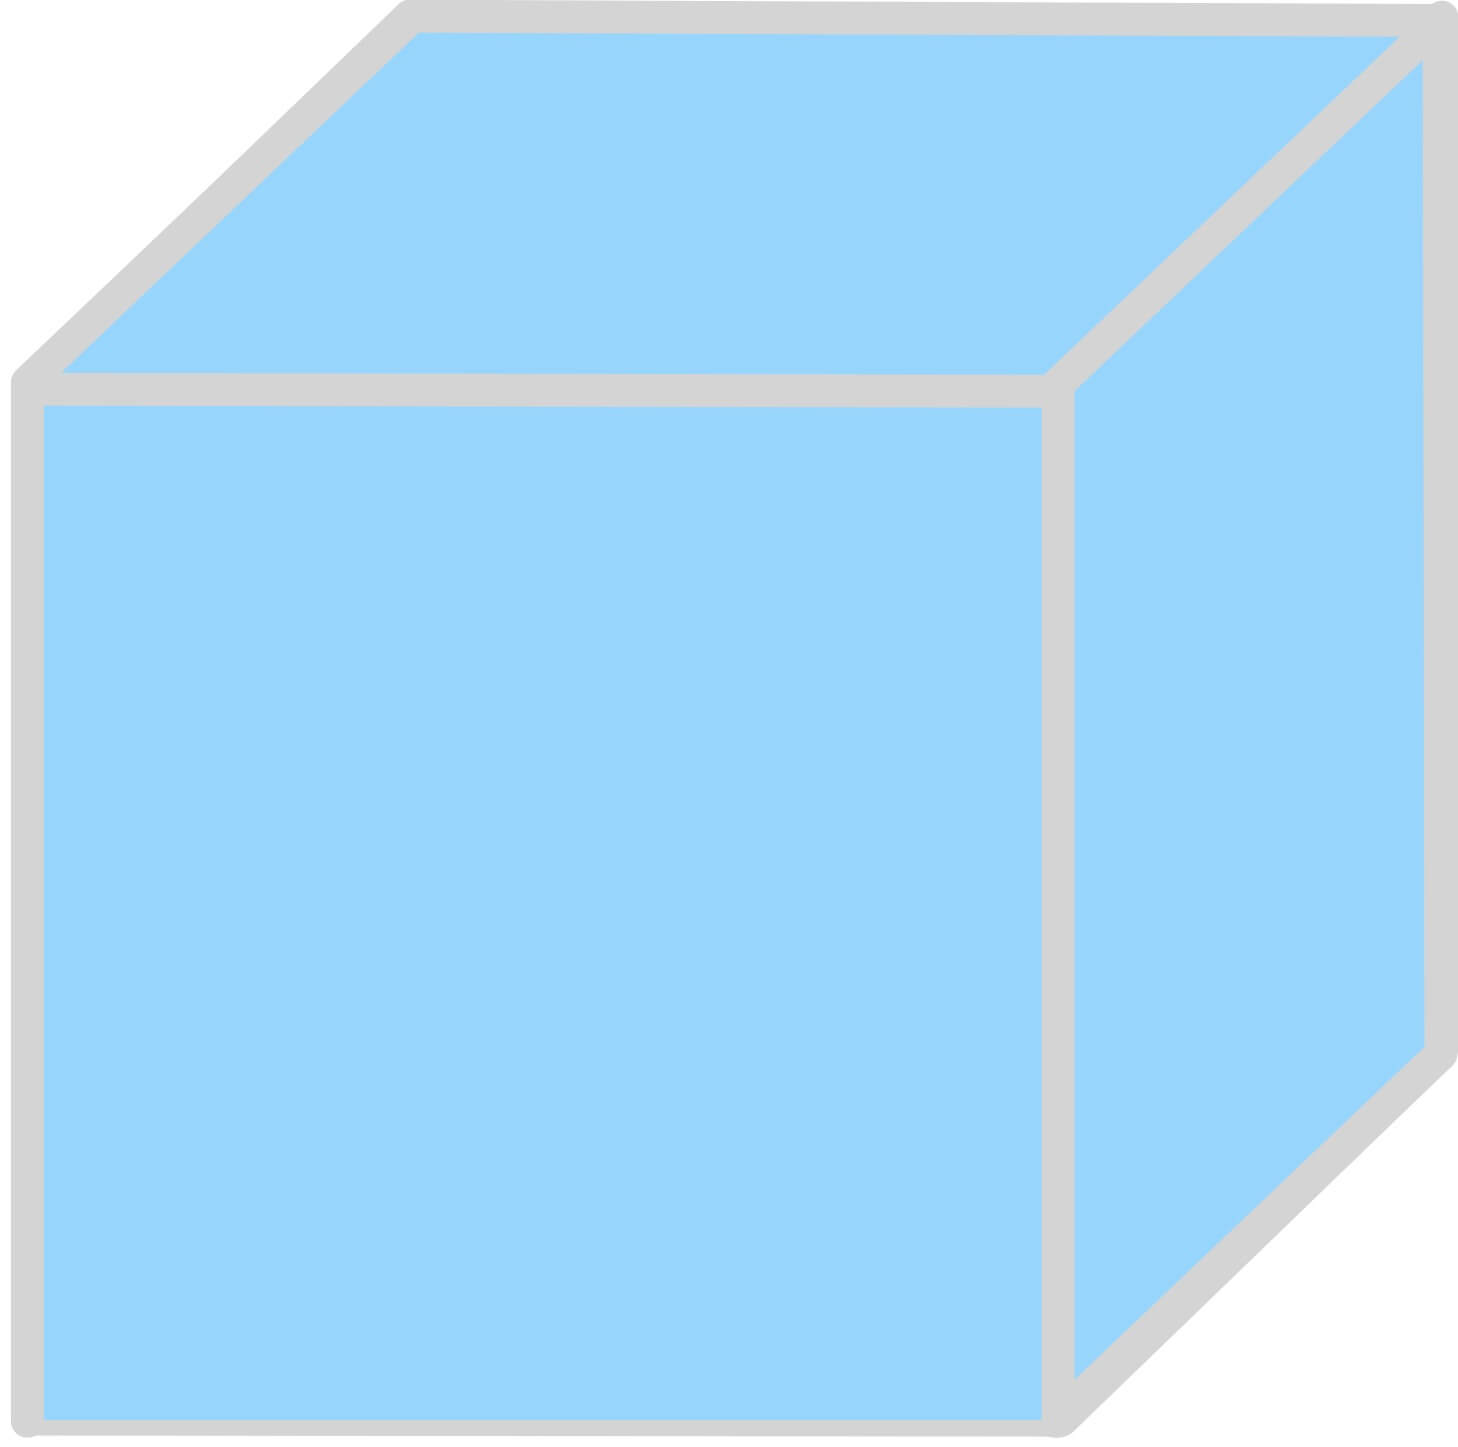
\includegraphics[width=0.5\textwidth]{calzone/26_calzone.jpg}
        \caption{\label{fig:calzone-diagram}The starch locations of the ``Calzone'' equivalence class}
    \end{figure}
\end{frame}

\begin{frame}{Examples of Calzone}
    \begin{tikzpicture}[remember picture,overlay]
        \node[xshift=-1.1cm,yshift=-2cm] at (current page.north east) {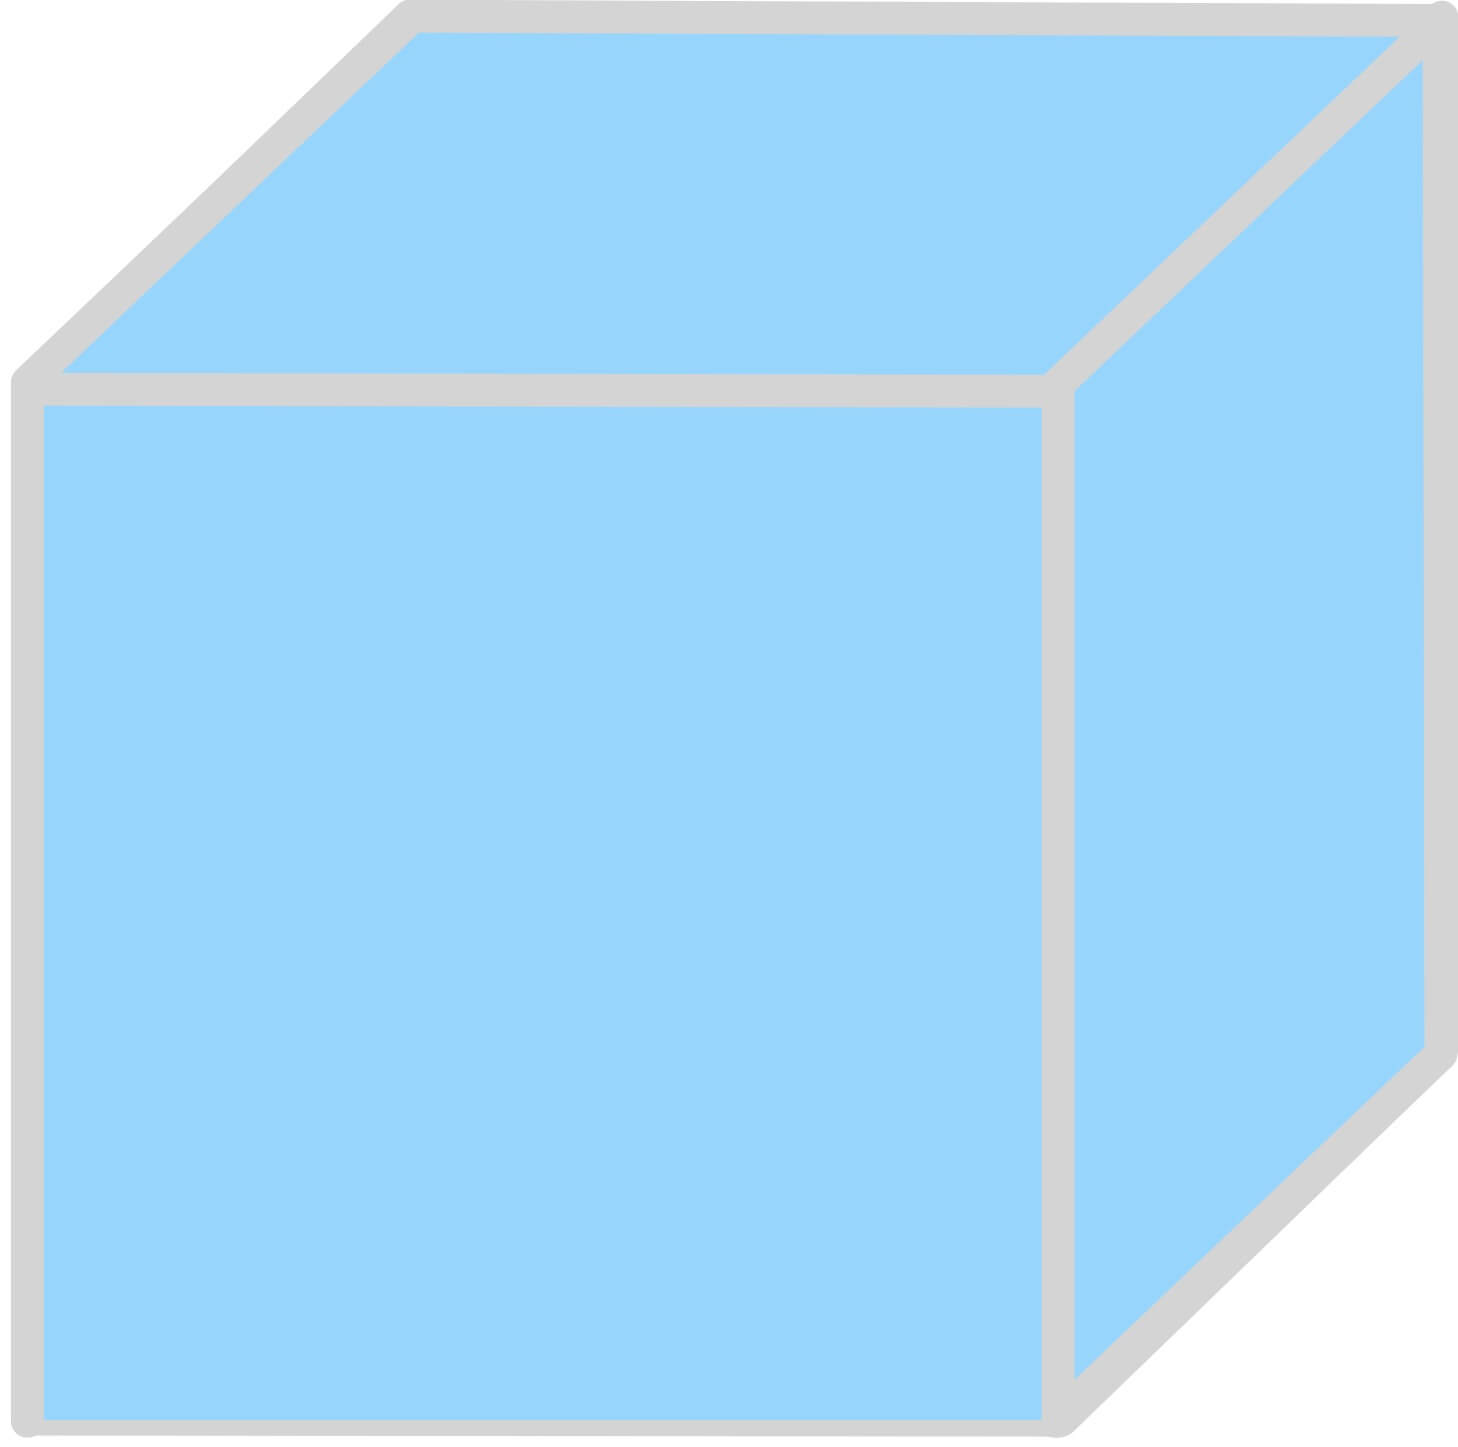
\includegraphics[width=0.1\textwidth]{calzone/26_calzone.jpg}};
    \end{tikzpicture}
    \begin{figure}
        \begin{subfigure}{.3\textwidth}
          \centering
          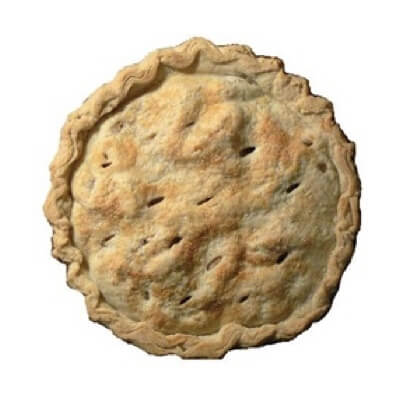
\includegraphics[width=.8\linewidth]{calzone/27_pie.jpg}
          \caption{\label{fig:whole-pie}Pie (whole)}
        \end{subfigure}
        \begin{subfigure}{.4\textwidth}
          \centering
          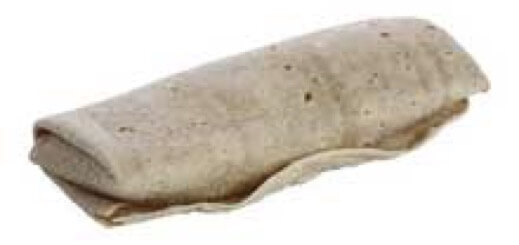
\includegraphics[width=.8\linewidth]{calzone/27_burrito.jpg}
          \caption{\label{fig:burrito}Burrito}
        \end{subfigure}%
        \begin{subfigure}{.4\textwidth}
          \centering
          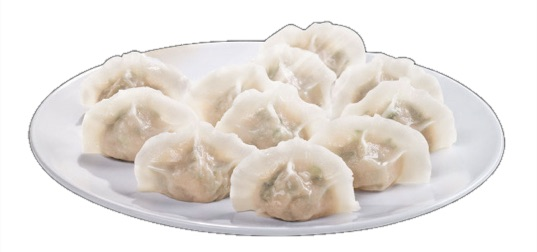
\includegraphics[width=.8\linewidth]{calzone/28_dumplings.jpg}
          \caption{\label{fig:dumplings}Dumplings}
        \end{subfigure}
    \end{figure}
\end{frame}

\begin{frame}{Is this enough?}
    \begin{itemize}
        \item For these groupings to be equivalence classes, their union must cover the entire set
        \item In the initial set of rulings, this is not true!
        \begin{itemize}
            \item For example foodstuffs with no starch, such as salads, are not in any of the groupings
        \end{itemize}
        \item To address this, we need to introduce a couple more classes to capture the foods which don't conform to our (beautiful) system
    \end{itemize}
\end{frame}

% Salad
\begin{frame}{The Cube Rule of Food -- Salad}
    \begin{figure}
        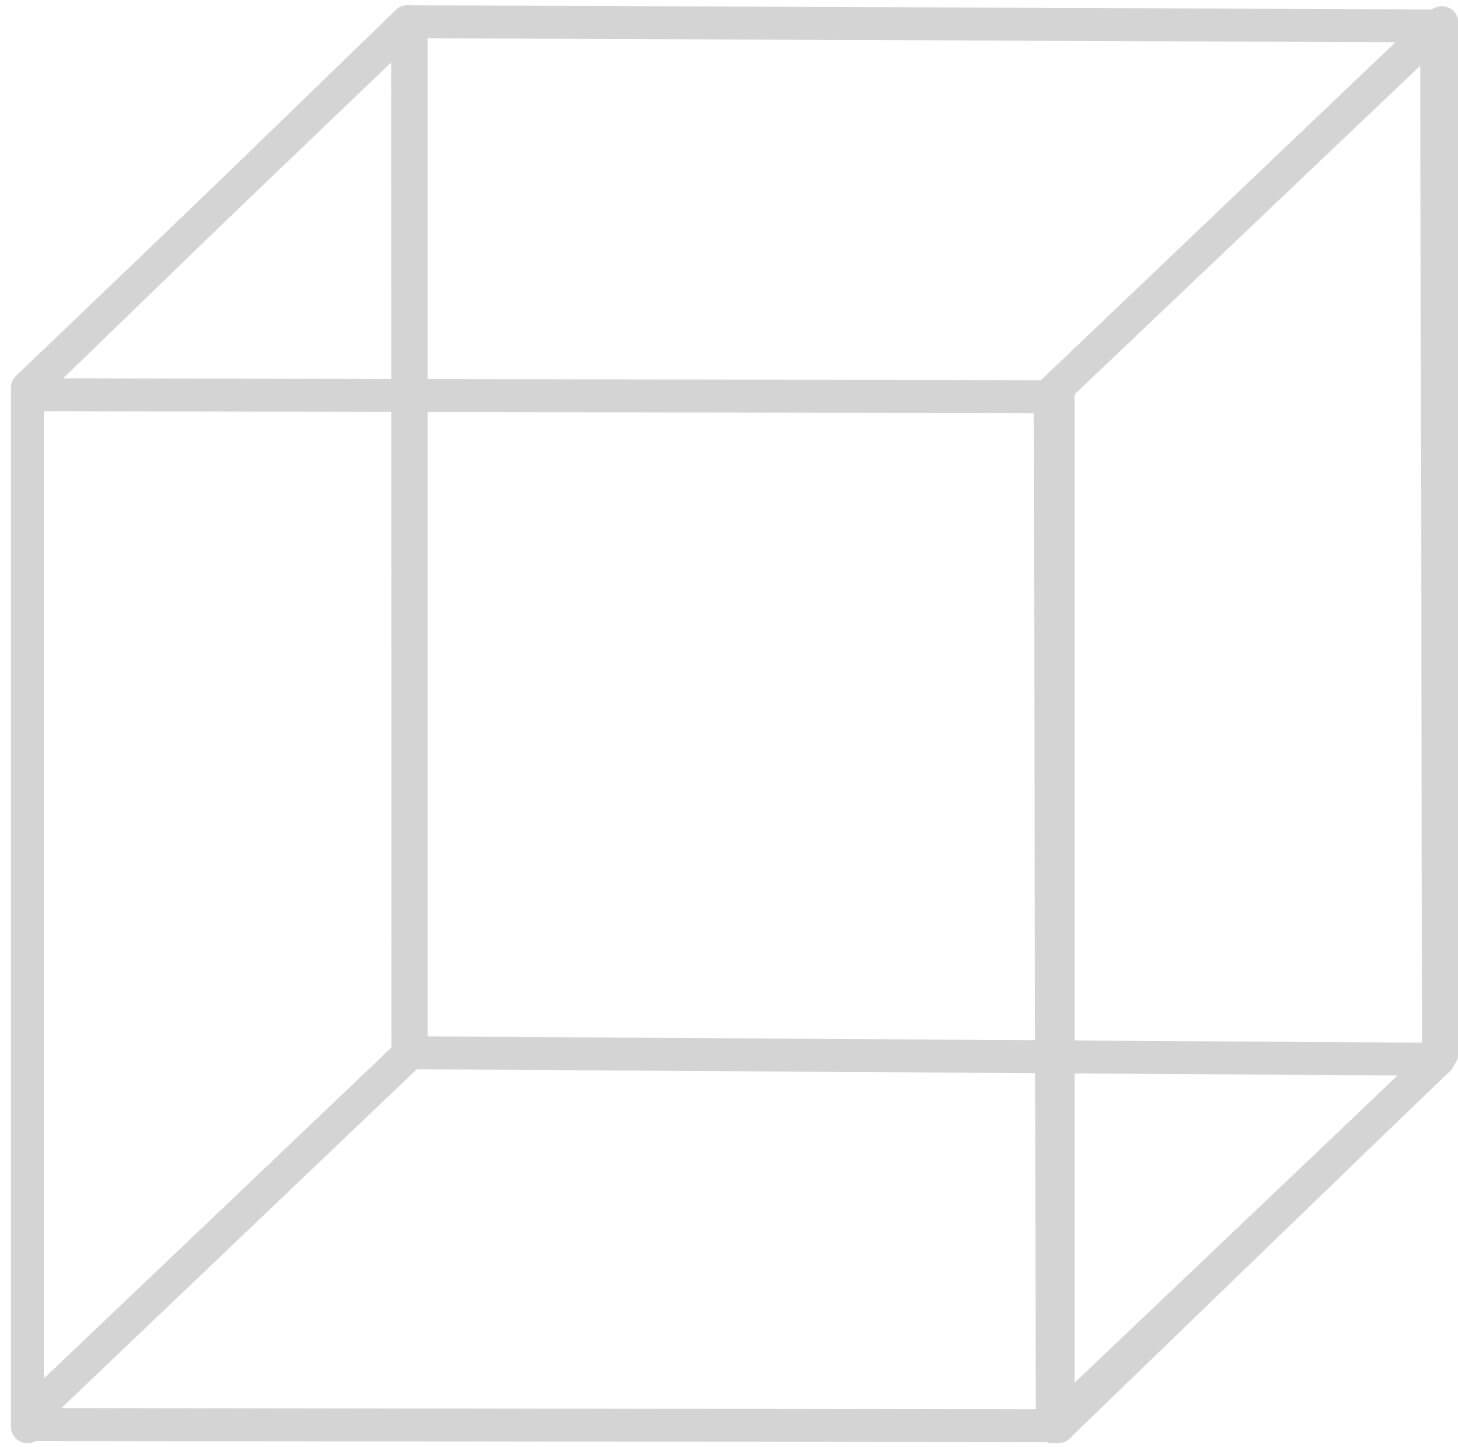
\includegraphics[width=0.5\textwidth]{salad/29_salad.jpg}
        \caption{\label{fig:salad-diagram}The starch locations of the ``Salad'' equivalence class}
    \end{figure}
\end{frame}

\begin{frame}{Examples of Salads}
    \begin{tikzpicture}[remember picture,overlay]
        \node[xshift=-1.1cm,yshift=-2cm] at (current page.north east) {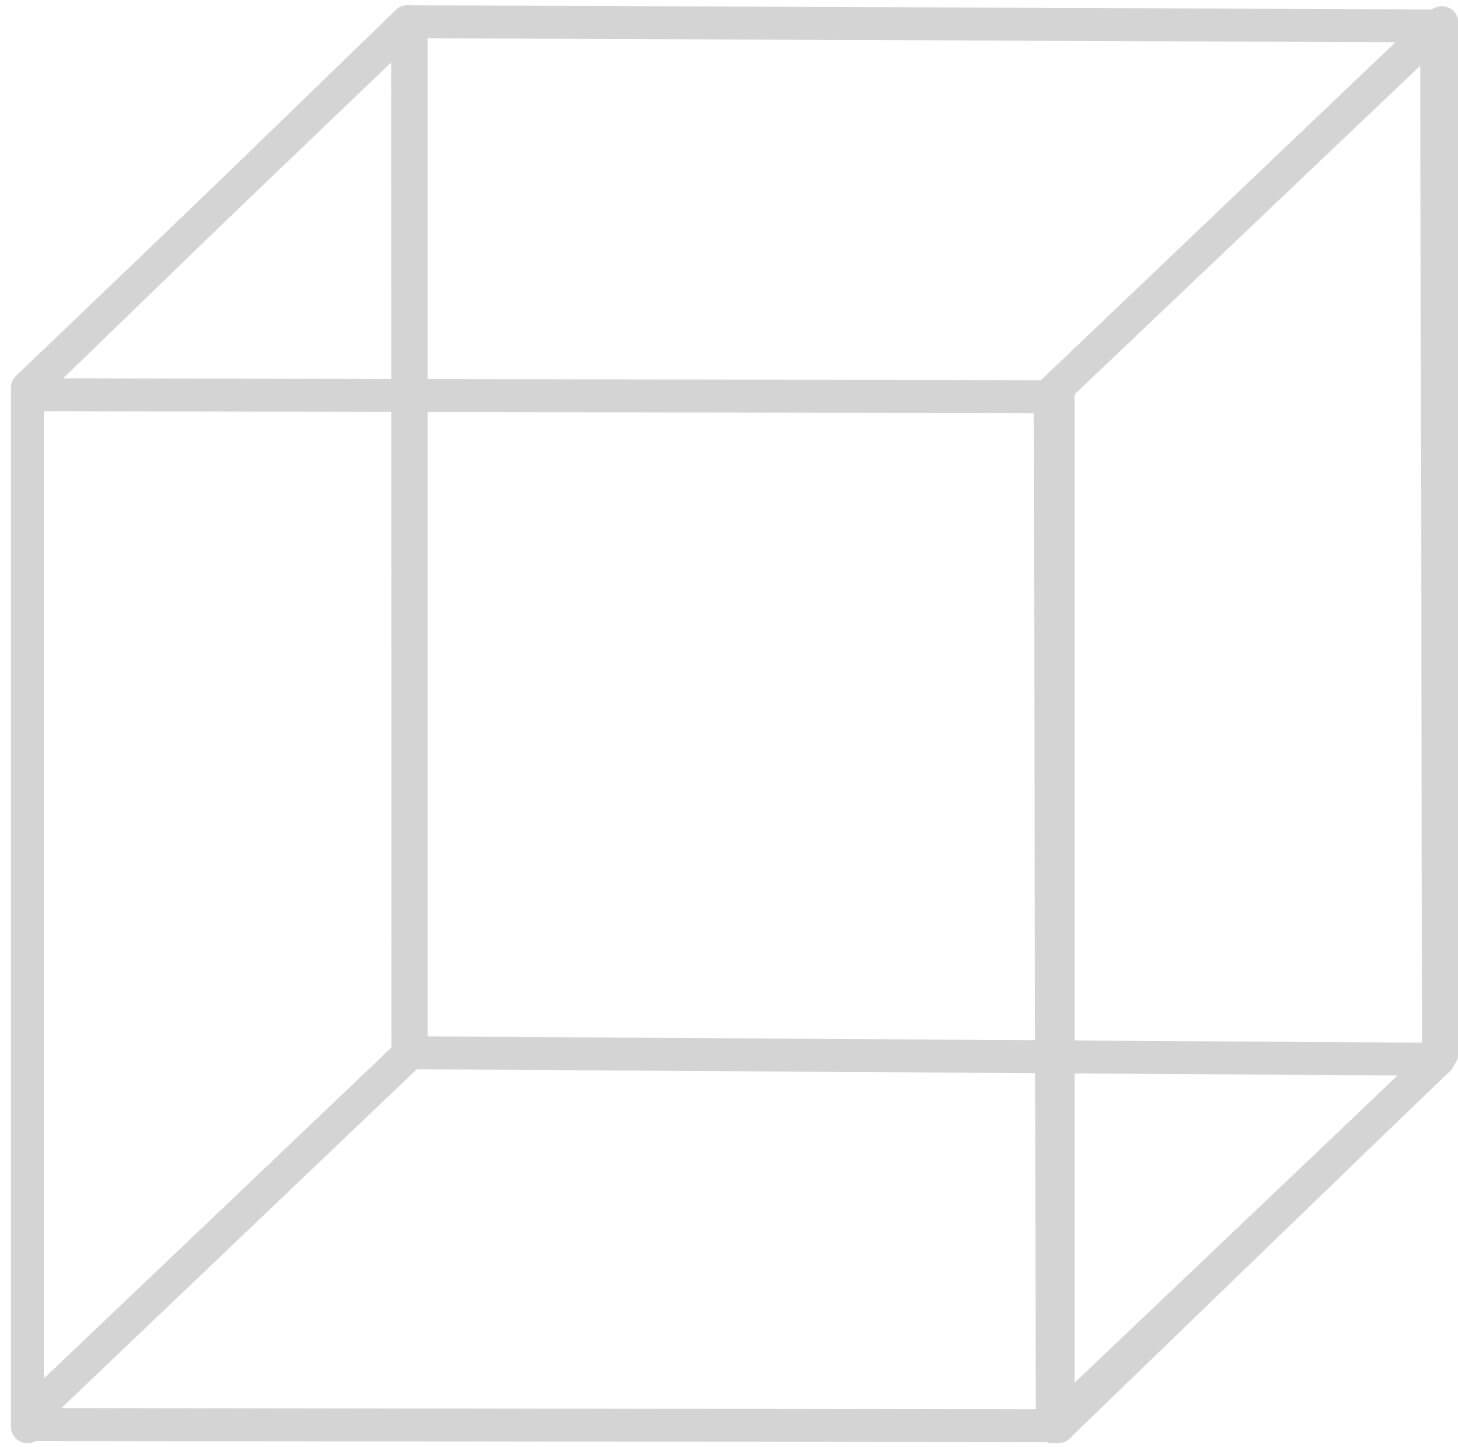
\includegraphics[width=0.1\textwidth]{salad/29_salad.jpg}};
    \end{tikzpicture}
    \begin{figure}
        \begin{subfigure}{.3\textwidth}
          \centering
          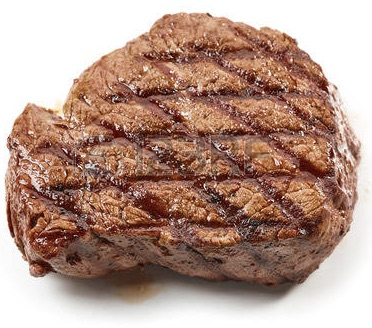
\includegraphics[width=.8\linewidth]{salad/30_steak.jpg}
          \caption{\label{fig:steak}Steak}
        \end{subfigure}
        \begin{subfigure}{.35\textwidth}
          \centering
          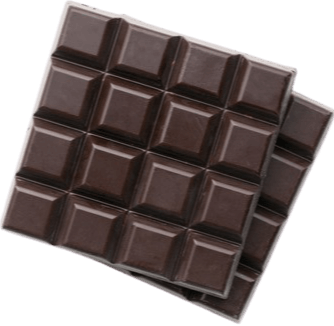
\includegraphics[width=.8\linewidth]{salad/31_chocolate.png}
          \caption{\label{fig:chocolate}Chocolate}
        \end{subfigure}%
        \begin{subfigure}{.35\textwidth}
          \centering
          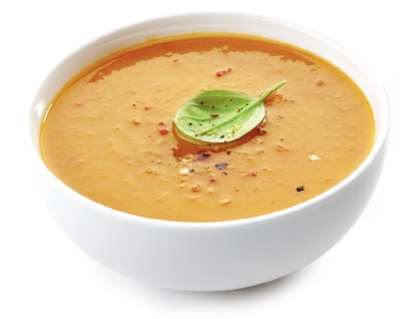
\includegraphics[width=.8\linewidth]{salad/31_soup.jpg}
          \caption{\label{fig:soup}Soup (wet salad)}
        \end{subfigure}
    \end{figure}
\end{frame}

% Nachos
\begin{frame}{The Cube Rule of Food -- Nachos}
    \begin{figure}
        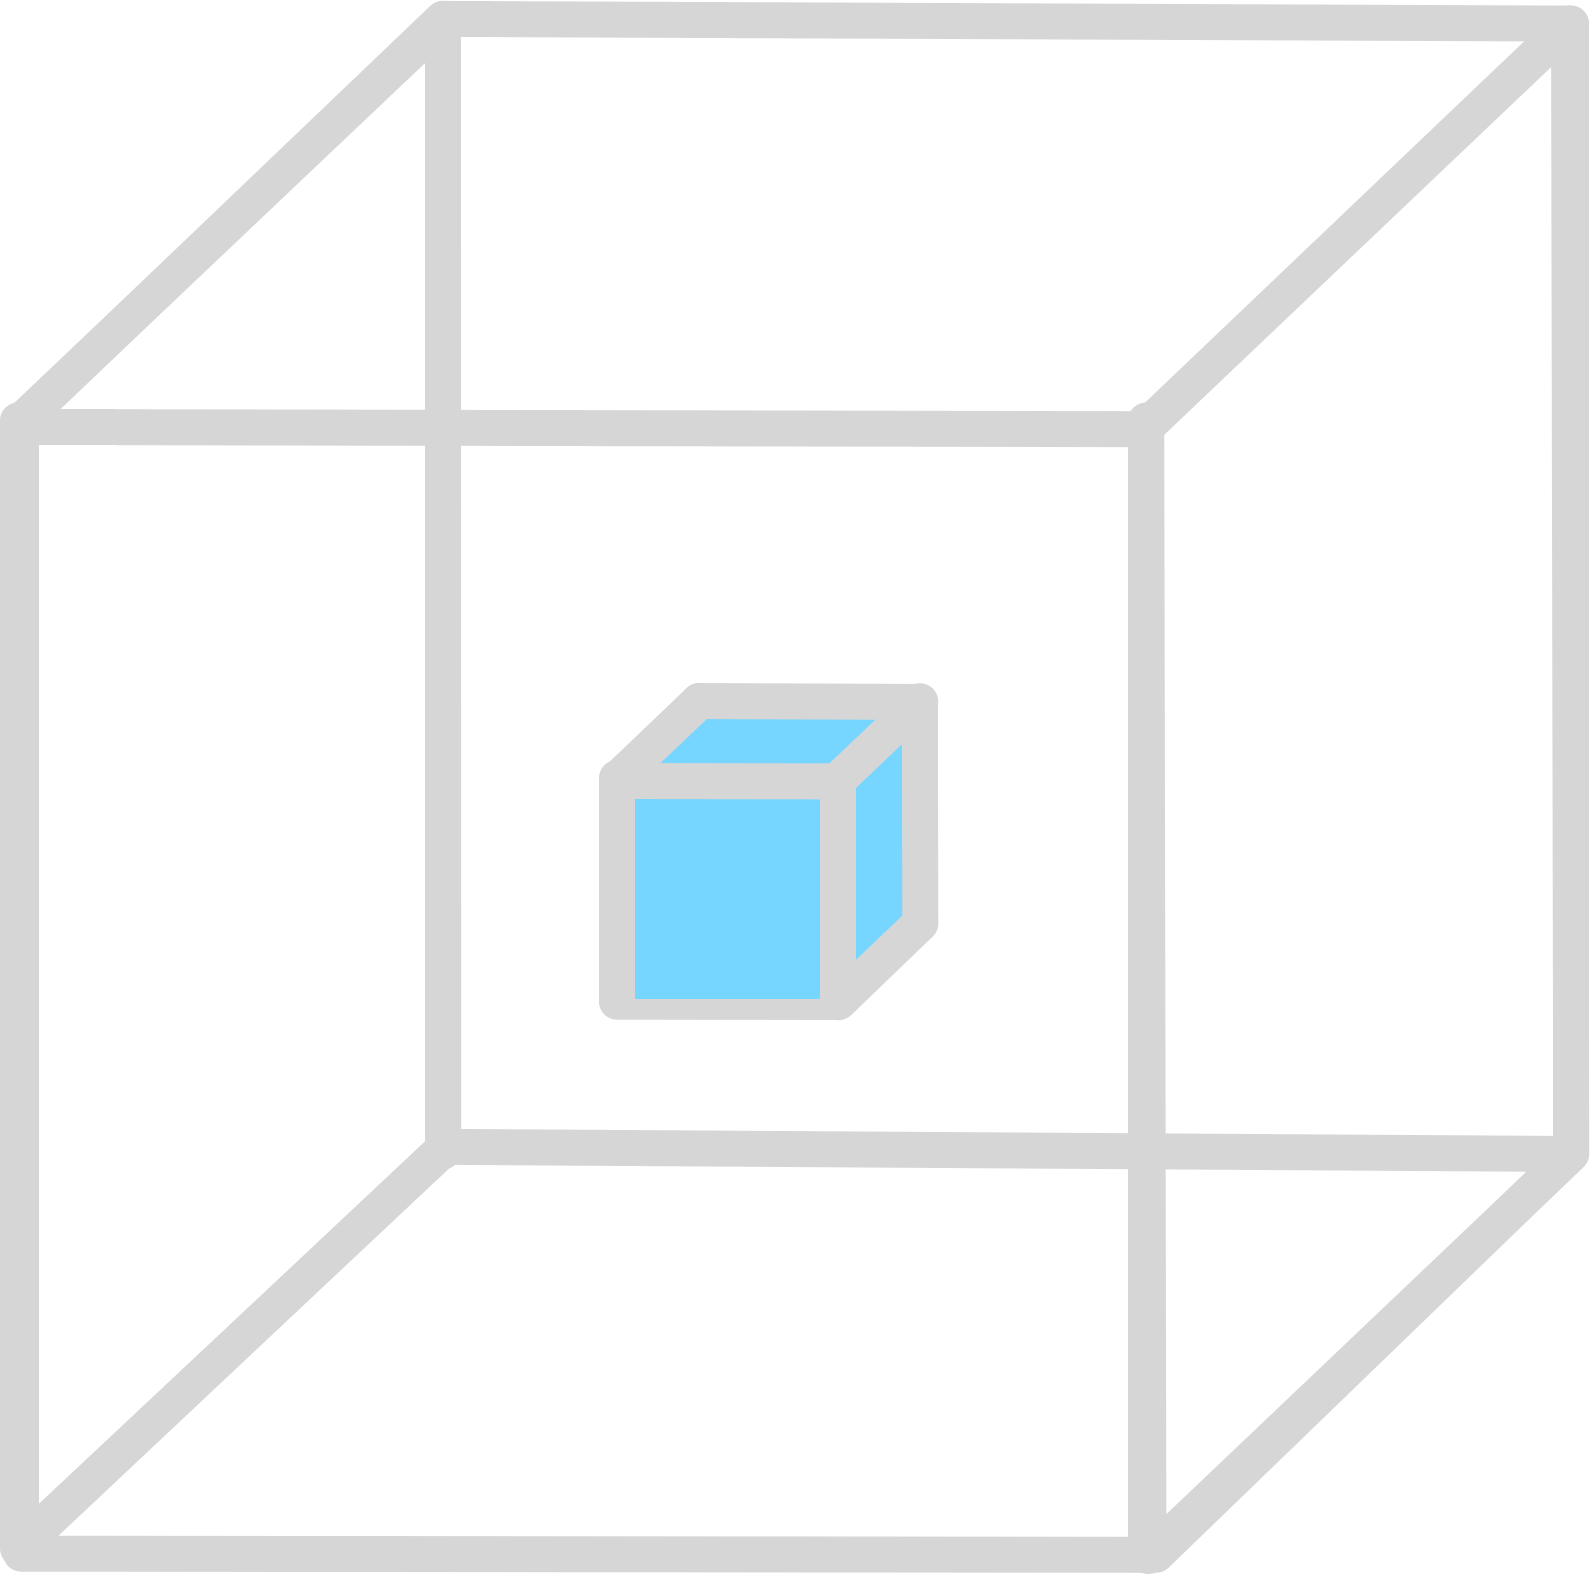
\includegraphics[width=0.5\textwidth]{nachos/34_nachos.png}
        \caption{\label{fig:nachos-diagram}The starch locations of the ``Nachos'' equivalence class}
    \end{figure}
\end{frame}

\begin{frame}{Examples of Nachos}
    \begin{tikzpicture}[remember picture,overlay]
        \node[xshift=-1.1cm,yshift=-2cm] at (current page.north east) {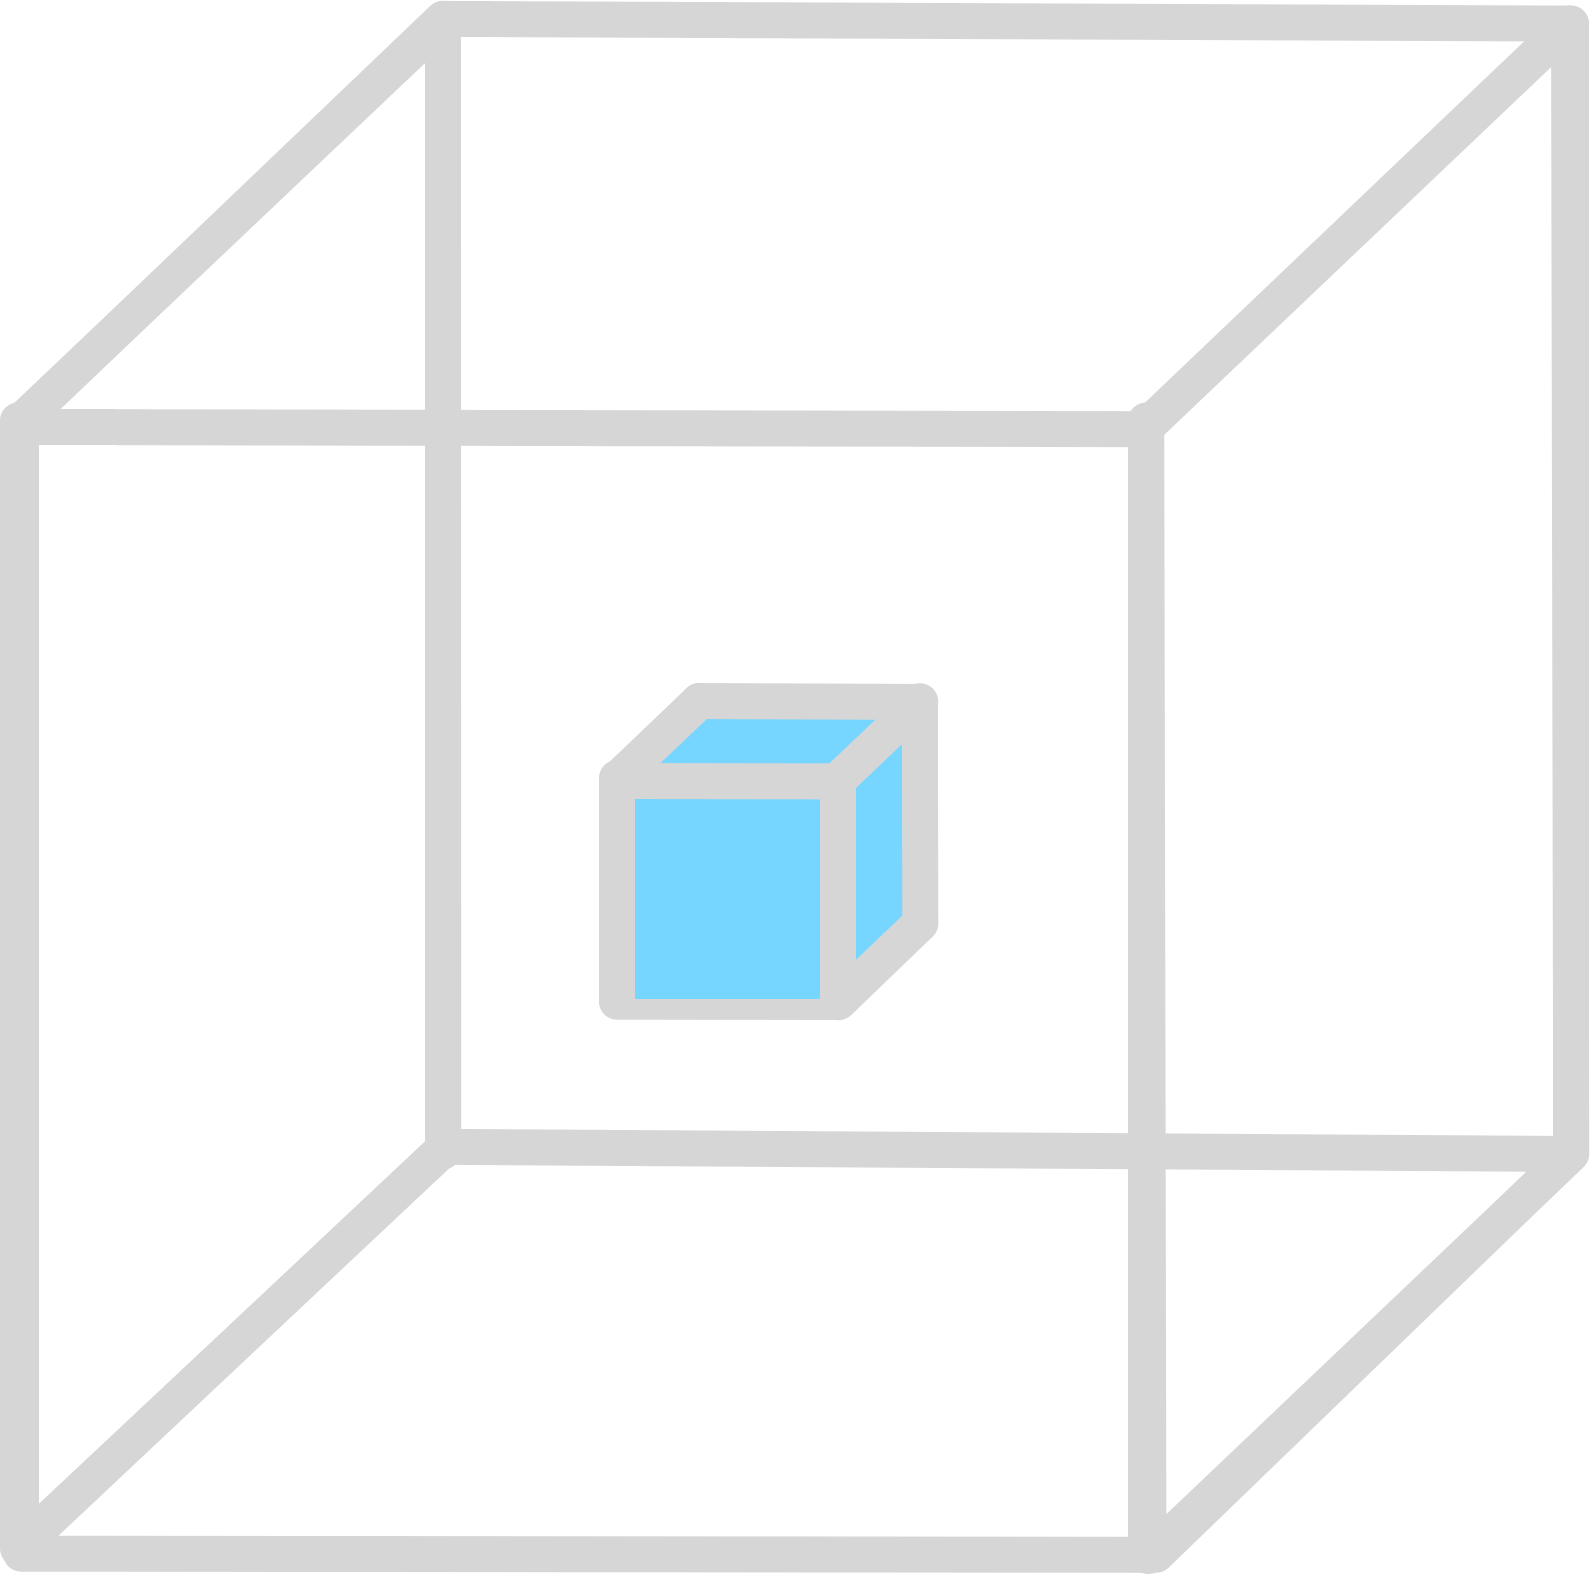
\includegraphics[width=0.1\textwidth]{nachos/34_nachos.png}};
    \end{tikzpicture}
    \begin{figure}
        \begin{subfigure}{.4\textwidth}
          \centering
          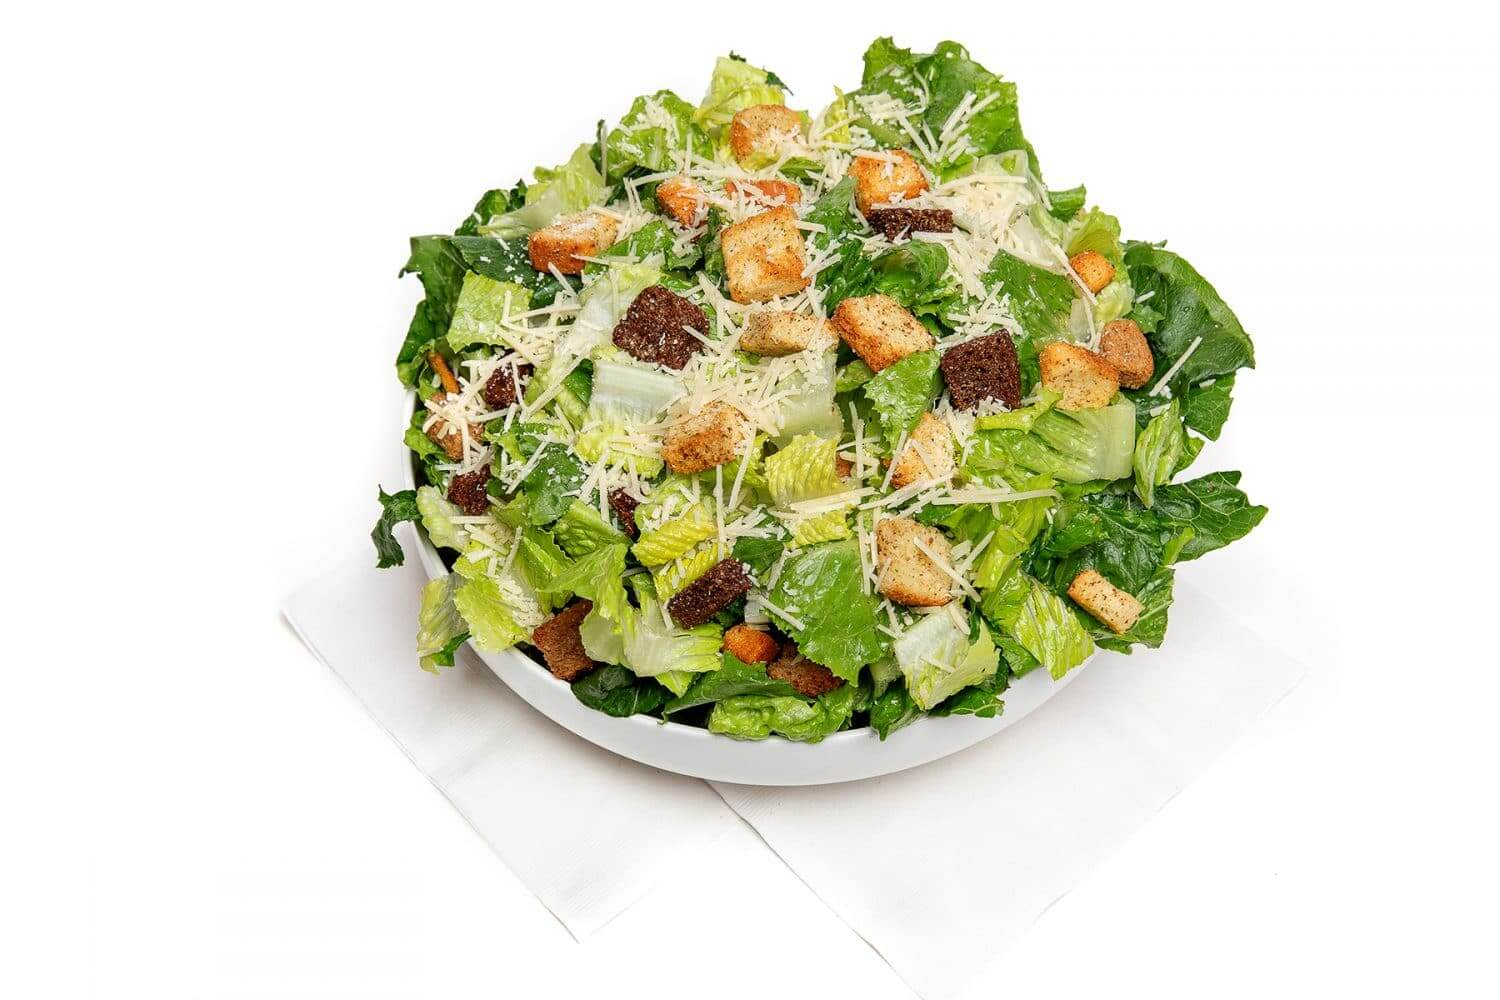
\includegraphics[width=\linewidth]{nachos/35_crouton_salad.jpg}
          \caption{\label{fig:crouton-salad}Salad (with croutons)}
        \end{subfigure}
        \begin{subfigure}{.5\textwidth}
          \centering
          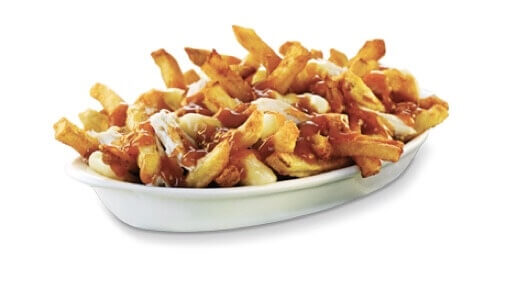
\includegraphics[width=.8\linewidth]{nachos/35_poutine.jpg}
          \caption{\label{fig:poutine}Poutine}
        \end{subfigure}
    \end{figure}
\end{frame}

% Cake
\begin{frame}{The Cube Rule of Food -- Cake}
    \begin{figure}
        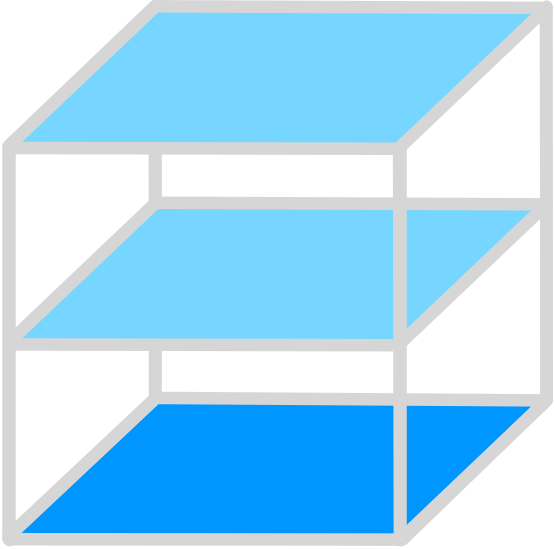
\includegraphics[width=0.5\textwidth]{cake/32_cake.png}
        \caption{\label{fig:cake-diagram}The starch locations of the ``Cake'' grouping of foodstuffs}
    \end{figure}
\end{frame}

\begin{frame}{Examples of Cakes}
    \begin{tikzpicture}[remember picture,overlay]
        \node[xshift=-1.1cm,yshift=-2cm] at (current page.north east) {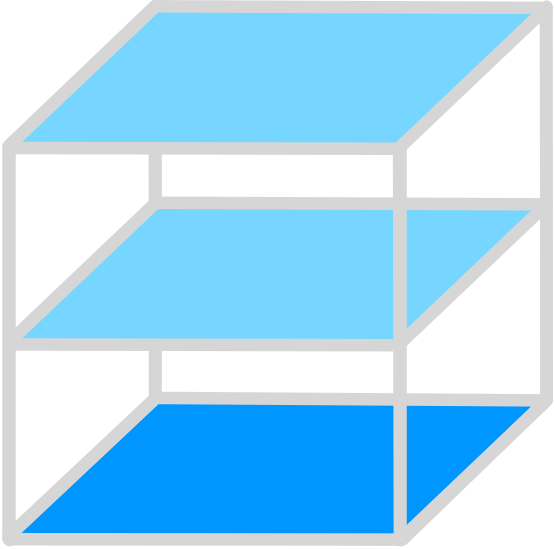
\includegraphics[width=0.1\textwidth]{cake/32_cake.png}};
    \end{tikzpicture}
    \begin{figure}
        \begin{subfigure}{.35\textwidth}
          \centering
          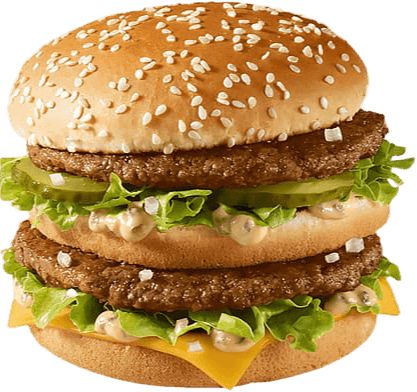
\includegraphics[width=\linewidth]{cake/33_big_mac.png}
          \caption{\label{fig:big-mac}Big Mac\texttrademark}
        \end{subfigure}
        \begin{subfigure}{.35\textwidth}
          \centering
          \includegraphics[width=.8\linewidth]{cake/33_flapjacks.png}
          \caption{\label{fig:pancake-stack}A stack of pancakes}
        \end{subfigure}
    \end{figure}
\end{frame}


\begin{frame}{Is \textit{\textbf{this}} enough?}
    \begin{itemize}
        \item I'm not sure how you would actually prove this!
        \item However, if you take a generous view of equivalence class membership, this is probably enough to uniquely cover all foods
    \end{itemize}
\end{frame}

% Questions for the audience?

\section{Part II - A (brief) introduction to Group Theory}

\begin{frame}{What is a group?}
    \begin{itemize}
        \item Intuitively, a group is an algebraic structure consisting of both:
        \vskip 1cm
        \begin{enumerate}
            \item A set of items
            \item An operation which combines two of its elements to form a third element
        \end{enumerate}
    \end{itemize}
\end{frame}

\begin{frame}{What is a group?}
    More formally, a group is defined as:
    \begin{itemize}
        \item A set of elements, $G$
        \item A binary operation $\bullet$ which maps two elements $a,b \in G$ to another element $c = a \bullet b \in G$ in the set
        \item Where the following properties hold:
        \begin{enumerate}
            \item \textbf{Closure} -- $\forall a,b \in G, \quad a \bullet b \in G$
            \item \textbf{Associativity} -- $\forall a,b,c \in G, \quad (a \bullet b) \bullet c = a \bullet (b \bullet c)$
            \item \textbf{Identity element} -- $\exists e \in G \forall a \in G, \quad e \bullet a = a \bullet e = a$
            \item \textbf{Inverse element} -- $\forall a \in G \exists b \in G, \quad a \bullet b = b \bullet a = e$
        \end{enumerate}
    \end{itemize}
\end{frame}

\begin{frame}{What if some of the properties don't hold?}
    \begin{figure}
        \includegraphics[width=0.6\textwidth]{algebraic_structures.png}
        \caption{\label{fig:algebraic-structures}Algebraic structures between magmas and groups \cite{ethaniel_english_2020}}
    \end{figure}
\end{frame}

\begin{frame}{Why are groups interesting?}
    Groups have many applications for understanding the Real World\texttrademark
    \begin{itemize}
        \item Modelling physical phenomena
        \begin{itemize}
            \item Crystals
            \item Hydrogen atoms
            \item Three of the four known fundamental forces in the universe
        \end{itemize}
        \item Public key cryptography
        \item And many more...\footnote{\href{https://tvtropes.org/pmwiki/pmwiki.php/Main/ChekhovsGun}{https://tvtropes.org/.../ChekhovsGun}}
    \end{itemize}
\end{frame}


\section{Part III - Defining Lasagne}


\begin{frame}
    \begin{figure}
        \includegraphics[width=0.6\textwidth]{Garfield_Loves_Lasagna.png}
        \caption{\label{fig:garfield-loves-lasagne}Garfield loves Lasagne \cite{garfield_lasagna}}
    \end{figure}
\end{frame}

\begin{frame}{What is a Lasagne?}
    \begin{figure}
        \includegraphics[width=0.5\textwidth]{lasagne_unstacked.png}
        \caption{\label{fig:lasagane-unstacked}A portion of Lasagne} %\cite{nast_lasagna_nodate}
    \end{figure}
\end{frame}

\begin{frame}{Is this still Lasagne?}
    \begin{figure}
        \begin{subfigure}{.3\textwidth}
          \centering
          \includegraphics[width=\linewidth]{lasagne_unstacked.png}
        \end{subfigure}
        \centering
        \qquad\tikz[baseline=-\baselineskip]\draw[ultra thick,->] (0,1) -- ++ (1,0);\quad
        \begin{subfigure}{.4\textwidth}
          \centering
          \includegraphics[width=.8\linewidth]{lasagne_stacked.png}
        \end{subfigure}
        \vskip 0.75cm
        \caption{\label{fig:lasagane-stacked}If you cut a portion of Lasagne in half, and stack one half on top of the other -- it is still Lasagne!}
    \end{figure}
\end{frame}

\begin{frame}{Does Lasagne form a group?}
    \begin{itemize}
        % \item An element in the set $G$ is a Lasagne with $n \in \mathbb{N}_{0}$ layers
        \item $G$ is the set containing all Lasagnes with a non-negative number of layers, i.e. $G = \{$ n-layer Lasagne $|\ n \in \mathbb{N}_{0}\}$
        % \begin{itemize}
        %     \item i.e. $G = \{$ n-layer Lasagne $|\ n \in \mathbb{N}_{0}\}$
        % \end{itemize} 
        \item The binary operation $\bullet$ is stacking two Lasagnes, one atop the other
        \vskip 1cm
        \item Do the four properties hold?
        \begin{enumerate}
            \item \textbf{Closure}
            \item \textbf{Associativity}
            \item \textbf{Identity element}
            \item \textbf{Inverse element}
        \end{enumerate}
    \end{itemize}
\end{frame}

\begin{frame}{Group properties of Lasagne?}
    \begin{itemize}
        \item<1-> Is Lasagne closed under the stacking operation?
        \begin{itemize}
            \item<2-> Yes! We have agreed if you stack two Lasagnes, one atop the other, the result is still Lasagne 
        \end{itemize}
        \item<3-> Is Lasagne associative under the stacking operation?
        \begin{itemize}
            \item<4-> Yes! The order in which you stack Lasagne doesn't matter -- it still ends up with the same number of layers at the end
        \end{itemize}
        \item<5-> Does Lasagne have an identity element under the stacking operation?
        \begin{itemize}
            \item<6-> Yes! The identity element is the empty Lasagne, a Lasagne with no layers
        \end{itemize}
        \item<7-> Does Lasagne have inverse elements under the stacking operation?
        \begin{itemize}
            \item<8-> No! By counter-example, there is no Lasagne with a non-negative integer number of layers which you could stack on a single-layer Lasagne to get the empty Lasagne
        \end{itemize}
    \end{itemize}
\end{frame}

% \begin{frame}{Closure?}
%     \textbf{Is Lasagne closed under the stacking operation?}
%     \begin{itemize}
%         \item Yes! We have agreed if you stack two Lasagnes, one atop the other, the result is still Lasagne 
%     \end{itemize}
% \end{frame}
% \begin{frame}{Associativity?}
%     \textbf{Is Lasagne associative under the stacking operation?}
%     \begin{itemize}
%         \item Yes! The order in which you stack Lasagne doesn't matter -- it still ends up with the same number of layers at the end
%     \end{itemize}
% \end{frame}
% \begin{frame}{Identity element?}
%     \textbf{Does Lasagne have an identity element under the stacking operation?}
%     \begin{itemize}
%         \item Yes! The identity element is the empty Lasagne, a Lasagne with no layers
%     \end{itemize}
% \end{frame}
% \begin{frame}{Inverse element?}
%     \texttt{Does Lasagne have inverse elements under the stacking operation?}
%     \begin{itemize}
%         \item No! By counter-example, there is no Lasagne with a non-negative integer number of layers which you could stack on a single-layer Lasagne to get the empty Lasagne
%     \end{itemize}
% \end{frame}

\begin{frame}{So what does it form?}
    \begin{figure}
        \includegraphics[width=0.6\textwidth]{algebraic_structures.png}
        \caption{\label{fig:algebraic-structures-2}Algebraic structures between magmas and groups \cite{ethaniel_english_2020}}
    \end{figure}
\end{frame}

\begin{frame}
    \begin{center}
        \Huge\textbf{Lasagne is a monoid under the stacking operation!}
    \end{center}
\end{frame}

\begin{frame}
    \begin{center}
        \Huge\textbf{Lasagne is a monoid under the stacking operation!}
        \vskip 2cm
        \small{However, it is not a monad, since it is not in the category of endofunctors...}
    \end{center}
\end{frame}

\begin{frame}[fragile]{The Lasagne monoid in Haskell}
    \begin{minted}[escapeinside=||]{haskell}
newtype Lasagne = Lasagne Int
    deriving (Show, Num)

-- The stacking operating can be considered integer 
-- addition of the number of layers
instance Semigroup Lasagne where
    (<>) = (+)

-- The identity element is the empty (zero-layer) Lasagne
instance Monoid Lasagne where
    mempty = Lasagne 0

-- Stacking 5 and 6 layers gives 11 layers:
--
-- ghci> Lasagne 5 <> Lasagne 6
-- Lasagne 11
    \end{minted}
\end{frame}


\begin{frame}{Extending the Cube Rule of Food}
    \begin{itemize}
        \item<1-> Now that we know Lasagne is a monoid, we can use it to extend the ``Cube Rule of Food''!
        \begin{itemize}
            \item Salad is isomorphic to the identity element of the Lasagne monoid
            \item Pizza is isomorphic to the single-layer element of the Lasagne monoid
            \item Sandwiches are isomorphic to the double-layer element in the monoid
            \vskip 0.5cm
            \item<2-> \textbf{In fact, Lasagne forms a rigorous definition of Cake!}
        \end{itemize}
    \end{itemize}
\end{frame}

\begin{frame}
    \begin{figure}
        \begin{subfigure}{.24\textwidth}
          \centering
          \includegraphics[width=\linewidth]{salad/29_salad.jpg}
          \caption{\label{fig:salad-lasagne}Salad as the identity Lasagne}
        \end{subfigure}
        \begin{subfigure}{.24\textwidth}
          \centering
          \includegraphics[width=\linewidth]{toast/16_toast.jpg}
          \caption{\label{fig:toast-lasagne}Toast as a single-layer Lasagne}
        \end{subfigure}
        \begin{subfigure}{.24\textwidth}
          \centering
          \includegraphics[width=\linewidth]{sandwich/18_sandwich.jpg}
          \caption{\label{fig:sandwich-lasagne}Sandwiches as a double-layer Lasagne}
        \end{subfigure}
        \begin{subfigure}{.24\textwidth}
          \centering
          \includegraphics[width=\linewidth]{cake/32_cake.png}
          \caption{\label{fig:cake-lasagne}Triple-layer cakes as a Lasagne}
        \end{subfigure}
        \caption{\label{fig:lasagne-subclasses}Other equivalence classes as elements of the Lasagne Monoid}
    \end{figure}
\end{frame}

\begin{frame}{Why is this useful?}
\end{frame}

\begin{frame}{Why is this useful?}
    \begin{center}
        \Huge\textbf{It isn't...}
    \end{center}
\end{frame}

\begin{frame}{Why is this useful?}
    \begin{center}
        \Huge\textbf{It isn't...}
        \vskip 2cm
        \small{But I think it is funny, and maybe you did too...}
    \end{center}
\end{frame}

\begin{frame}
    \begin{tikzpicture}[remember picture,overlay]
        \node[xshift=-1.1cm,yshift=-1.3cm] at (current page.north east) {\includegraphics[width=0.15\textwidth]{qr-code.png}};
    \end{tikzpicture}
    \begin{center}
        \Huge\textbf{Thanks for listening!} \\
        \vskip 1cm
        \pause
        \Large\textit{I refuse to answer any questions...}
    \end{center}
\end{frame}


% \begin{frame}[allowframebreaks]{Bibliography}
%         \nocite{*}
%         \bibliographystyle{IEEEtran}
%         \bibliography{citations.bib}
% \end{frame}

\begin{frame}[t,allowframebreaks]
\frametitle{Bibliography}
\printbibliography[heading=none]
\end{frame}

\end{document}
